% Created by tikzDevice version 0.7.0 on 2014-06-30 20:14:13
% !TEX encoding = UTF-8 Unicode
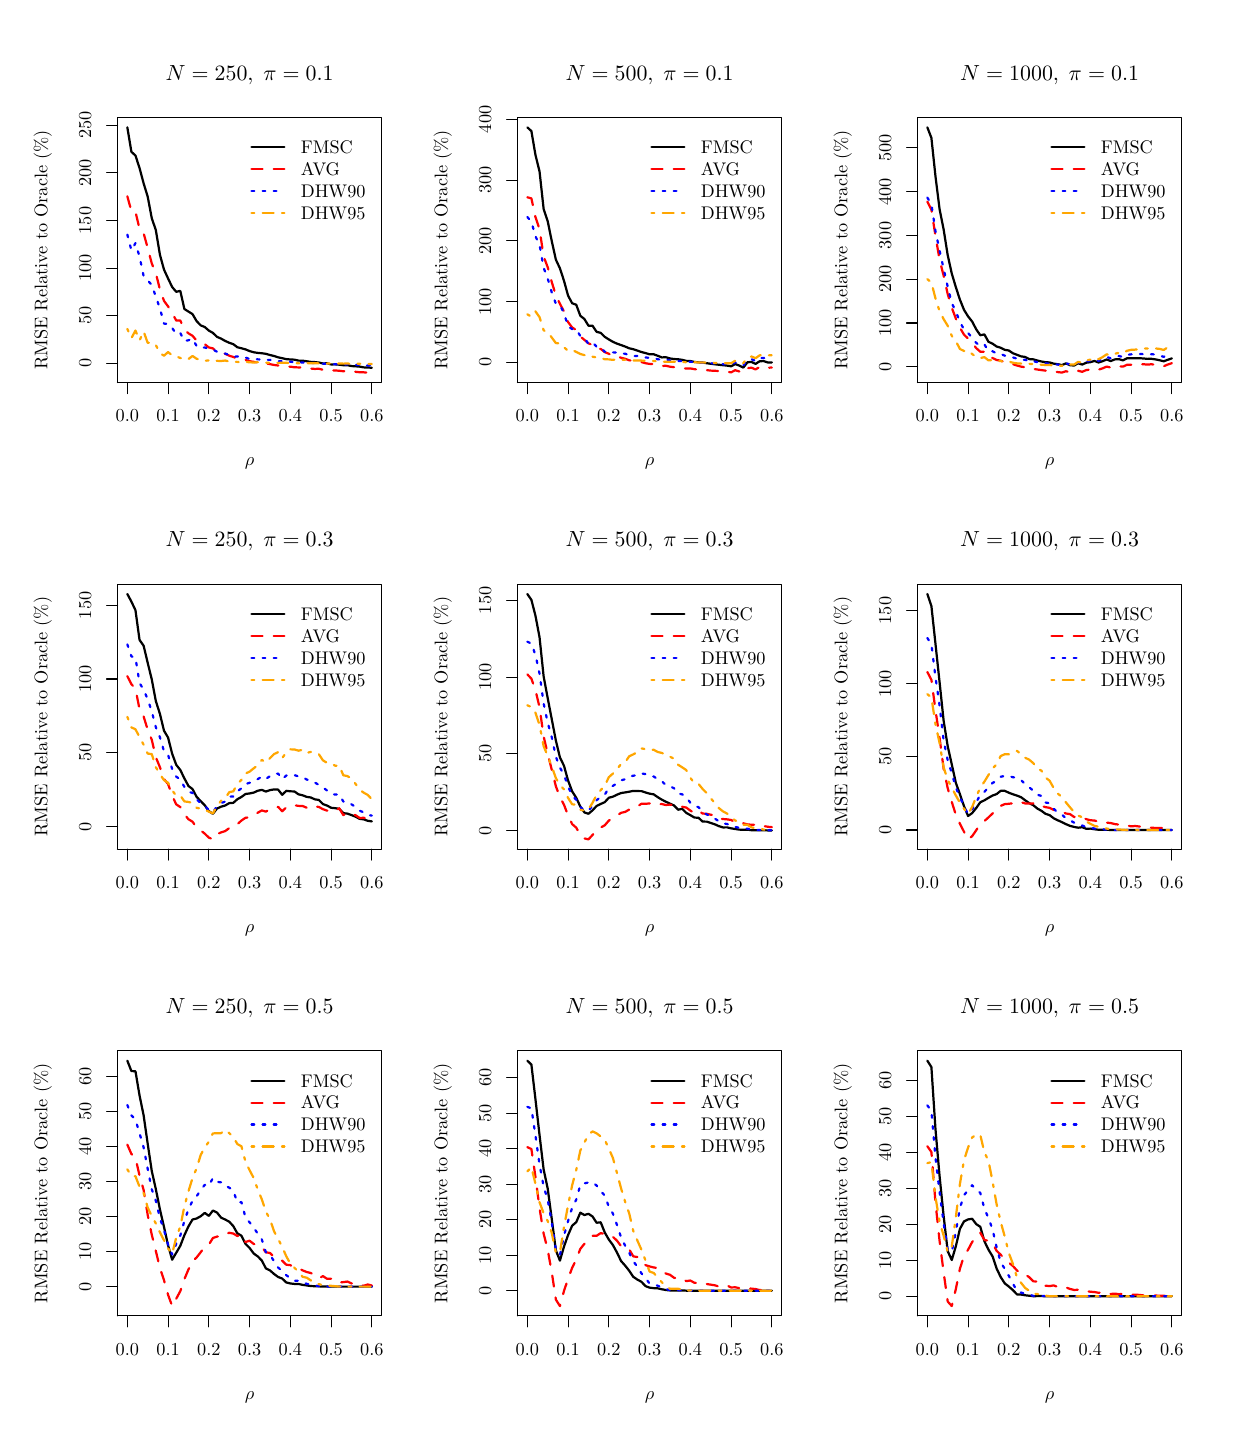
\begin{tikzpicture}[x=1pt,y=1pt]
\definecolor[named]{fillColor}{rgb}{1.00,1.00,1.00}
\path[use as bounding box,fill=fillColor,fill opacity=0.00] (0,0) rectangle (433.62,505.89);
\begin{scope}
\path[clip] ( 32.47,377.65) rectangle (127.91,473.42);
\definecolor[named]{drawColor}{rgb}{0.00,0.00,0.00}

\path[draw=drawColor,line width= 0.8pt,line join=round,line cap=round] ( 36.01,469.87) --
	( 37.48,461.02) --
	( 38.95,459.68) --
	( 40.42,455.18) --
	( 41.90,449.62) --
	( 43.37,444.83) --
	( 44.84,437.05) --
	( 46.32,432.69) --
	( 47.79,423.83) --
	( 49.26,418.46) --
	( 50.73,415.27) --
	( 52.21,412.17) --
	( 53.68,410.44) --
	( 55.15,410.77) --
	( 56.63,404.22) --
	( 58.10,403.30) --
	( 59.57,402.38) --
	( 61.04,399.86) --
	( 62.52,398.31) --
	( 63.99,397.72) --
	( 65.46,396.42) --
	( 66.93,395.60) --
	( 68.41,394.16) --
	( 69.88,393.53) --
	( 71.35,392.70) --
	( 72.83,392.03) --
	( 74.30,391.51) --
	( 75.77,390.40) --
	( 77.24,390.04) --
	( 78.72,389.63) --
	( 80.19,389.02) --
	( 81.66,388.60) --
	( 83.14,388.36) --
	( 84.61,388.24) --
	( 86.08,388.03) --
	( 87.55,387.60) --
	( 89.03,387.24) --
	( 90.50,386.76) --
	( 91.97,386.45) --
	( 93.44,386.11) --
	( 94.92,385.99) --
	( 96.39,385.92) --
	( 97.86,385.58) --
	( 99.34,385.54) --
	(100.81,385.35) --
	(102.28,385.11) --
	(103.75,385.04) --
	(105.23,384.88) --
	(106.70,384.54) --
	(108.17,384.62) --
	(109.65,384.19) --
	(111.12,384.23) --
	(112.59,384.10) --
	(114.06,383.91) --
	(115.54,383.93) --
	(117.01,383.60) --
	(118.48,383.52) --
	(119.95,383.41) --
	(121.43,383.13) --
	(122.90,383.09) --
	(124.37,382.99);
\end{scope}
\begin{scope}
\path[clip] (  0.00,  0.00) rectangle (433.62,505.89);
\definecolor[named]{drawColor}{rgb}{0.00,0.00,0.00}

\path[draw=drawColor,line width= 0.4pt,line join=round,line cap=round] ( 36.01,377.65) -- (124.37,377.65);

\path[draw=drawColor,line width= 0.4pt,line join=round,line cap=round] ( 36.01,377.65) -- ( 36.01,373.69);

\path[draw=drawColor,line width= 0.4pt,line join=round,line cap=round] ( 50.73,377.65) -- ( 50.73,373.69);

\path[draw=drawColor,line width= 0.4pt,line join=round,line cap=round] ( 65.46,377.65) -- ( 65.46,373.69);

\path[draw=drawColor,line width= 0.4pt,line join=round,line cap=round] ( 80.19,377.65) -- ( 80.19,373.69);

\path[draw=drawColor,line width= 0.4pt,line join=round,line cap=round] ( 94.92,377.65) -- ( 94.92,373.69);

\path[draw=drawColor,line width= 0.4pt,line join=round,line cap=round] (109.65,377.65) -- (109.65,373.69);

\path[draw=drawColor,line width= 0.4pt,line join=round,line cap=round] (124.37,377.65) -- (124.37,373.69);

\node[text=drawColor,anchor=base,inner sep=0pt, outer sep=0pt, scale=  0.66] at ( 36.01,363.40) {0.0};

\node[text=drawColor,anchor=base,inner sep=0pt, outer sep=0pt, scale=  0.66] at ( 50.73,363.40) {0.1};

\node[text=drawColor,anchor=base,inner sep=0pt, outer sep=0pt, scale=  0.66] at ( 65.46,363.40) {0.2};

\node[text=drawColor,anchor=base,inner sep=0pt, outer sep=0pt, scale=  0.66] at ( 80.19,363.40) {0.3};

\node[text=drawColor,anchor=base,inner sep=0pt, outer sep=0pt, scale=  0.66] at ( 94.92,363.40) {0.4};

\node[text=drawColor,anchor=base,inner sep=0pt, outer sep=0pt, scale=  0.66] at (109.65,363.40) {0.5};

\node[text=drawColor,anchor=base,inner sep=0pt, outer sep=0pt, scale=  0.66] at (124.37,363.40) {0.6};

\path[draw=drawColor,line width= 0.4pt,line join=round,line cap=round] ( 32.47,384.61) -- ( 32.47,470.63);

\path[draw=drawColor,line width= 0.4pt,line join=round,line cap=round] ( 32.47,384.61) -- ( 28.51,384.61);

\path[draw=drawColor,line width= 0.4pt,line join=round,line cap=round] ( 32.47,401.82) -- ( 28.51,401.82);

\path[draw=drawColor,line width= 0.4pt,line join=round,line cap=round] ( 32.47,419.02) -- ( 28.51,419.02);

\path[draw=drawColor,line width= 0.4pt,line join=round,line cap=round] ( 32.47,436.23) -- ( 28.51,436.23);

\path[draw=drawColor,line width= 0.4pt,line join=round,line cap=round] ( 32.47,453.43) -- ( 28.51,453.43);

\path[draw=drawColor,line width= 0.4pt,line join=round,line cap=round] ( 32.47,470.63) -- ( 28.51,470.63);

\node[text=drawColor,rotate= 90.00,anchor=base,inner sep=0pt, outer sep=0pt, scale=  0.66] at ( 22.97,384.61) {0};

\node[text=drawColor,rotate= 90.00,anchor=base,inner sep=0pt, outer sep=0pt, scale=  0.66] at ( 22.97,401.82) {50};

\node[text=drawColor,rotate= 90.00,anchor=base,inner sep=0pt, outer sep=0pt, scale=  0.66] at ( 22.97,419.02) {100};

\node[text=drawColor,rotate= 90.00,anchor=base,inner sep=0pt, outer sep=0pt, scale=  0.66] at ( 22.97,436.23) {150};

\node[text=drawColor,rotate= 90.00,anchor=base,inner sep=0pt, outer sep=0pt, scale=  0.66] at ( 22.97,453.43) {200};

\node[text=drawColor,rotate= 90.00,anchor=base,inner sep=0pt, outer sep=0pt, scale=  0.66] at ( 22.97,470.63) {250};

\path[draw=drawColor,line width= 0.4pt,line join=round,line cap=round] ( 32.47,377.65) --
	(127.91,377.65) --
	(127.91,473.42) --
	( 32.47,473.42) --
	( 32.47,377.65);
\end{scope}
\begin{scope}
\path[clip] (  0.00,337.26) rectangle (144.54,505.89);
\definecolor[named]{drawColor}{rgb}{0.00,0.00,0.00}

\node[text=drawColor,anchor=base,inner sep=0pt, outer sep=0pt, scale=  0.79] at ( 80.19,486.92) {\bfseries $N=250, \;\pi=0.1$};

\node[text=drawColor,anchor=base,inner sep=0pt, outer sep=0pt, scale=  0.66] at ( 80.19,347.56) {$\rho$};

\node[text=drawColor,rotate= 90.00,anchor=base,inner sep=0pt, outer sep=0pt, scale=  0.66] at (  7.13,425.53) {RMSE Relative to Oracle (\%)};
\end{scope}
\begin{scope}
\path[clip] ( 32.47,377.65) rectangle (127.91,473.42);
\definecolor[named]{drawColor}{rgb}{1.00,0.00,0.00}

\path[draw=drawColor,line width= 0.8pt,dash pattern=on 4pt off 4pt ,line join=round,line cap=round] ( 36.01,444.95) --
	( 37.48,439.59) --
	( 38.95,439.36) --
	( 40.42,433.19) --
	( 41.90,431.57) --
	( 43.37,426.28) --
	( 44.84,420.70) --
	( 46.32,417.12) --
	( 47.79,411.30) --
	( 49.26,407.17) --
	( 50.73,405.16) --
	( 52.21,402.83) --
	( 53.68,400.04) --
	( 55.15,400.08) --
	( 56.63,396.67) --
	( 58.10,395.44) --
	( 59.57,394.54) --
	( 61.04,392.83) --
	( 62.52,392.12) --
	( 63.99,391.50) --
	( 65.46,390.34) --
	( 66.93,389.99) --
	( 68.41,388.74) --
	( 69.88,388.24) --
	( 71.35,388.06) --
	( 72.83,387.35) --
	( 74.30,386.89) --
	( 75.77,386.33) --
	( 77.24,385.95) --
	( 78.72,385.81) --
	( 80.19,385.36) --
	( 81.66,385.13) --
	( 83.14,384.88) --
	( 84.61,384.66) --
	( 86.08,384.57) --
	( 87.55,384.31) --
	( 89.03,384.00) --
	( 90.50,383.81) --
	( 91.97,383.61) --
	( 93.44,383.43) --
	( 94.92,383.39) --
	( 96.39,383.17) --
	( 97.86,383.12) --
	( 99.34,383.07) --
	(100.81,382.83) --
	(102.28,382.71) --
	(103.75,382.57) --
	(105.23,382.64) --
	(106.70,382.25) --
	(108.17,382.33) --
	(109.65,382.07) --
	(111.12,382.02) --
	(112.59,381.91) --
	(114.06,381.73) --
	(115.54,381.91) --
	(117.01,381.56) --
	(118.48,381.53) --
	(119.95,381.37) --
	(121.43,381.35) --
	(122.90,381.20) --
	(124.37,381.22);
\definecolor[named]{drawColor}{rgb}{0.00,0.00,1.00}

\path[draw=drawColor,line width= 0.8pt,dash pattern=on 1pt off 3pt ,line join=round,line cap=round] ( 36.01,431.12) --
	( 37.48,425.40) --
	( 38.95,428.03) --
	( 40.42,423.17) --
	( 41.90,416.12) --
	( 43.37,414.56) --
	( 44.84,412.89) --
	( 46.32,408.60) --
	( 47.79,404.44) --
	( 49.26,398.95) --
	( 50.73,398.83) --
	( 52.21,397.37) --
	( 53.68,395.20) --
	( 55.15,395.55) --
	( 56.63,392.64) --
	( 58.10,392.94) --
	( 59.57,393.44) --
	( 61.04,390.87) --
	( 62.52,390.05) --
	( 63.99,390.33) --
	( 65.46,389.81) --
	( 66.93,389.55) --
	( 68.41,388.82) --
	( 69.88,388.31) --
	( 71.35,388.12) --
	( 72.83,387.64) --
	( 74.30,386.92) --
	( 75.77,387.11) --
	( 77.24,386.64) --
	( 78.72,386.69) --
	( 80.19,386.15) --
	( 81.66,386.31) --
	( 83.14,386.03) --
	( 84.61,385.99) --
	( 86.08,385.84) --
	( 87.55,385.85) --
	( 89.03,385.57) --
	( 90.50,385.38) --
	( 91.97,385.37) --
	( 93.44,385.14) --
	( 94.92,385.16) --
	( 96.39,385.02) --
	( 97.86,384.94) --
	( 99.34,384.88) --
	(100.81,384.93) --
	(102.28,384.69) --
	(103.75,384.76) --
	(105.23,384.59) --
	(106.70,384.47) --
	(108.17,384.47) --
	(109.65,384.33) --
	(111.12,384.26) --
	(112.59,384.25) --
	(114.06,384.17) --
	(115.54,384.22) --
	(117.01,384.02) --
	(118.48,384.02) --
	(119.95,383.98) --
	(121.43,383.80) --
	(122.90,383.82) --
	(124.37,383.75);
\definecolor[named]{drawColor}{rgb}{1.00,0.65,0.00}

\path[draw=drawColor,line width= 0.8pt,dash pattern=on 1pt off 3pt on 4pt off 3pt ,line join=round,line cap=round] ( 36.01,397.03) --
	( 37.48,393.70) --
	( 38.95,396.44) --
	( 40.42,392.87) --
	( 41.90,396.11) --
	( 43.37,391.97) --
	( 44.84,392.18) --
	( 46.32,391.16) --
	( 47.79,388.27) --
	( 49.26,387.35) --
	( 50.73,388.66) --
	( 52.21,387.47) --
	( 53.68,387.06) --
	( 55.15,386.54) --
	( 56.63,385.84) --
	( 58.10,386.14) --
	( 59.57,387.27) --
	( 61.04,386.24) --
	( 62.52,385.92) --
	( 63.99,385.50) --
	( 65.46,385.67) --
	( 66.93,385.92) --
	( 68.41,385.50) --
	( 69.88,385.43) --
	( 71.35,385.60) --
	( 72.83,385.25) --
	( 74.30,385.15) --
	( 75.77,385.12) --
	( 77.24,384.94) --
	( 78.72,385.16) --
	( 80.19,384.96) --
	( 81.66,384.91) --
	( 83.14,384.99) --
	( 84.61,384.85) --
	( 86.08,384.81) --
	( 87.55,384.79) --
	( 89.03,384.79) --
	( 90.50,384.75) --
	( 91.97,384.79) --
	( 93.44,384.80) --
	( 94.92,384.67) --
	( 96.39,384.70) --
	( 97.86,384.61) --
	( 99.34,384.69) --
	(100.81,384.67) --
	(102.28,384.63) --
	(103.75,384.61) --
	(105.23,384.58) --
	(106.70,384.55) --
	(108.17,384.55) --
	(109.65,384.51) --
	(111.12,384.51) --
	(112.59,384.53) --
	(114.06,384.49) --
	(115.54,384.51) --
	(117.01,384.46) --
	(118.48,384.46) --
	(119.95,384.46) --
	(121.43,384.34) --
	(122.90,384.37) --
	(124.37,384.36);
\definecolor[named]{drawColor}{rgb}{0.00,0.00,0.00}

\path[draw=drawColor,line width= 0.8pt,line join=round,line cap=round] ( 80.89,462.63) -- ( 92.77,462.63);
\definecolor[named]{drawColor}{rgb}{1.00,0.00,0.00}

\path[draw=drawColor,line width= 0.8pt,dash pattern=on 4pt off 4pt ,line join=round,line cap=round] ( 80.89,454.71) -- ( 92.77,454.71);
\definecolor[named]{drawColor}{rgb}{0.00,0.00,1.00}

\path[draw=drawColor,line width= 0.8pt,dash pattern=on 1pt off 3pt ,line join=round,line cap=round] ( 80.89,446.79) -- ( 92.77,446.79);
\definecolor[named]{drawColor}{rgb}{1.00,0.65,0.00}

\path[draw=drawColor,line width= 0.8pt,dash pattern=on 1pt off 3pt on 4pt off 3pt ,line join=round,line cap=round] ( 80.89,438.87) -- ( 92.77,438.87);
\definecolor[named]{drawColor}{rgb}{0.00,0.00,0.00}

\node[text=drawColor,anchor=base west,inner sep=0pt, outer sep=0pt, scale=  0.66] at ( 98.71,460.35) {FMSC};

\node[text=drawColor,anchor=base west,inner sep=0pt, outer sep=0pt, scale=  0.66] at ( 98.71,452.43) {AVG};

\node[text=drawColor,anchor=base west,inner sep=0pt, outer sep=0pt, scale=  0.66] at ( 98.71,444.51) {DHW90};

\node[text=drawColor,anchor=base west,inner sep=0pt, outer sep=0pt, scale=  0.66] at ( 98.71,436.59) {DHW95};
\end{scope}
\begin{scope}
\path[clip] (177.01,377.65) rectangle (272.45,473.42);
\definecolor[named]{drawColor}{rgb}{0.00,0.00,0.00}

\path[draw=drawColor,line width= 0.8pt,line join=round,line cap=round] (180.55,469.87) --
	(182.02,468.51) --
	(183.49,459.88) --
	(184.96,453.93) --
	(186.44,440.39) --
	(187.91,435.96) --
	(189.38,428.74) --
	(190.86,422.06) --
	(192.33,418.92) --
	(193.80,414.41) --
	(195.27,409.06) --
	(196.75,406.30) --
	(198.22,405.76) --
	(199.69,401.80) --
	(201.17,400.60) --
	(202.64,398.20) --
	(204.11,398.19) --
	(205.58,395.98) --
	(207.06,395.60) --
	(208.53,394.16) --
	(210.00,393.23) --
	(211.47,392.37) --
	(212.95,391.71) --
	(214.42,391.20) --
	(215.89,390.66) --
	(217.37,390.03) --
	(218.84,389.69) --
	(220.31,389.20) --
	(221.78,388.68) --
	(223.26,388.30) --
	(224.73,387.86) --
	(226.20,387.87) --
	(227.68,387.32) --
	(229.15,386.73) --
	(230.62,386.80) --
	(232.09,386.36) --
	(233.57,386.15) --
	(235.04,386.06) --
	(236.51,385.86) --
	(237.98,385.49) --
	(239.46,385.41) --
	(240.93,385.10) --
	(242.40,384.94) --
	(243.88,384.87) --
	(245.35,384.64) --
	(246.82,384.43) --
	(248.29,384.25) --
	(249.77,384.08) --
	(251.24,383.92) --
	(252.71,383.77) --
	(254.19,383.52) --
	(255.66,384.33) --
	(257.13,383.79) --
	(258.60,383.06) --
	(260.08,384.97) --
	(261.55,385.10) --
	(263.02,384.39) --
	(264.50,385.35) --
	(265.97,385.41) --
	(267.44,384.91) --
	(268.91,384.92);
\end{scope}
\begin{scope}
\path[clip] (  0.00,  0.00) rectangle (433.62,505.89);
\definecolor[named]{drawColor}{rgb}{0.00,0.00,0.00}

\path[draw=drawColor,line width= 0.4pt,line join=round,line cap=round] (180.55,377.65) -- (268.91,377.65);

\path[draw=drawColor,line width= 0.4pt,line join=round,line cap=round] (180.55,377.65) -- (180.55,373.69);

\path[draw=drawColor,line width= 0.4pt,line join=round,line cap=round] (195.27,377.65) -- (195.27,373.69);

\path[draw=drawColor,line width= 0.4pt,line join=round,line cap=round] (210.00,377.65) -- (210.00,373.69);

\path[draw=drawColor,line width= 0.4pt,line join=round,line cap=round] (224.73,377.65) -- (224.73,373.69);

\path[draw=drawColor,line width= 0.4pt,line join=round,line cap=round] (239.46,377.65) -- (239.46,373.69);

\path[draw=drawColor,line width= 0.4pt,line join=round,line cap=round] (254.19,377.65) -- (254.19,373.69);

\path[draw=drawColor,line width= 0.4pt,line join=round,line cap=round] (268.91,377.65) -- (268.91,373.69);

\node[text=drawColor,anchor=base,inner sep=0pt, outer sep=0pt, scale=  0.66] at (180.55,363.40) {0.0};

\node[text=drawColor,anchor=base,inner sep=0pt, outer sep=0pt, scale=  0.66] at (195.27,363.40) {0.1};

\node[text=drawColor,anchor=base,inner sep=0pt, outer sep=0pt, scale=  0.66] at (210.00,363.40) {0.2};

\node[text=drawColor,anchor=base,inner sep=0pt, outer sep=0pt, scale=  0.66] at (224.73,363.40) {0.3};

\node[text=drawColor,anchor=base,inner sep=0pt, outer sep=0pt, scale=  0.66] at (239.46,363.40) {0.4};

\node[text=drawColor,anchor=base,inner sep=0pt, outer sep=0pt, scale=  0.66] at (254.19,363.40) {0.5};

\node[text=drawColor,anchor=base,inner sep=0pt, outer sep=0pt, scale=  0.66] at (268.91,363.40) {0.6};

\path[draw=drawColor,line width= 0.4pt,line join=round,line cap=round] (177.01,384.93) -- (177.01,472.75);

\path[draw=drawColor,line width= 0.4pt,line join=round,line cap=round] (177.01,384.93) -- (173.05,384.93);

\path[draw=drawColor,line width= 0.4pt,line join=round,line cap=round] (177.01,406.89) -- (173.05,406.89);

\path[draw=drawColor,line width= 0.4pt,line join=round,line cap=round] (177.01,428.84) -- (173.05,428.84);

\path[draw=drawColor,line width= 0.4pt,line join=round,line cap=round] (177.01,450.80) -- (173.05,450.80);

\path[draw=drawColor,line width= 0.4pt,line join=round,line cap=round] (177.01,472.75) -- (173.05,472.75);

\node[text=drawColor,rotate= 90.00,anchor=base,inner sep=0pt, outer sep=0pt, scale=  0.66] at (167.51,384.93) {0};

\node[text=drawColor,rotate= 90.00,anchor=base,inner sep=0pt, outer sep=0pt, scale=  0.66] at (167.51,406.89) {100};

\node[text=drawColor,rotate= 90.00,anchor=base,inner sep=0pt, outer sep=0pt, scale=  0.66] at (167.51,428.84) {200};

\node[text=drawColor,rotate= 90.00,anchor=base,inner sep=0pt, outer sep=0pt, scale=  0.66] at (167.51,450.80) {300};

\node[text=drawColor,rotate= 90.00,anchor=base,inner sep=0pt, outer sep=0pt, scale=  0.66] at (167.51,472.75) {400};

\path[draw=drawColor,line width= 0.4pt,line join=round,line cap=round] (177.01,377.65) --
	(272.45,377.65) --
	(272.45,473.42) --
	(177.01,473.42) --
	(177.01,377.65);
\end{scope}
\begin{scope}
\path[clip] (144.54,337.26) rectangle (289.08,505.89);
\definecolor[named]{drawColor}{rgb}{0.00,0.00,0.00}

\node[text=drawColor,anchor=base,inner sep=0pt, outer sep=0pt, scale=  0.79] at (224.73,486.92) {\bfseries $N=500, \;\pi=0.1$};

\node[text=drawColor,anchor=base,inner sep=0pt, outer sep=0pt, scale=  0.66] at (224.73,347.56) {$\rho$};

\node[text=drawColor,rotate= 90.00,anchor=base,inner sep=0pt, outer sep=0pt, scale=  0.66] at (151.67,425.53) {RMSE Relative to Oracle (\%)};
\end{scope}
\begin{scope}
\path[clip] (177.01,377.65) rectangle (272.45,473.42);
\definecolor[named]{drawColor}{rgb}{1.00,0.00,0.00}

\path[draw=drawColor,line width= 0.8pt,dash pattern=on 4pt off 4pt ,line join=round,line cap=round] (180.55,444.61) --
	(182.02,444.18) --
	(183.49,437.41) --
	(184.96,433.02) --
	(186.44,423.23) --
	(187.91,419.33) --
	(189.38,413.96) --
	(190.86,409.15) --
	(192.33,406.10) --
	(193.80,403.35) --
	(195.27,399.51) --
	(196.75,397.54) --
	(198.22,396.66) --
	(199.69,394.28) --
	(201.17,393.08) --
	(202.64,391.80) --
	(204.11,391.26) --
	(205.58,389.92) --
	(207.06,389.80) --
	(208.53,388.63) --
	(210.00,388.05) --
	(211.47,387.19) --
	(212.95,387.17) --
	(214.42,386.61) --
	(215.89,386.24) --
	(217.37,385.69) --
	(218.84,385.49) --
	(220.31,385.33) --
	(221.78,385.06) --
	(223.26,384.63) --
	(224.73,384.39) --
	(226.20,384.35) --
	(227.68,383.95) --
	(229.15,383.63) --
	(230.62,383.72) --
	(232.09,383.38) --
	(233.57,383.21) --
	(235.04,383.07) --
	(236.51,382.97) --
	(237.98,382.69) --
	(239.46,382.74) --
	(240.93,382.49) --
	(242.40,382.26) --
	(243.88,382.29) --
	(245.35,382.14) --
	(246.82,381.97) --
	(248.29,381.89) --
	(249.77,381.83) --
	(251.24,381.66) --
	(252.71,381.54) --
	(254.19,381.34) --
	(255.66,382.11) --
	(257.13,381.66) --
	(258.60,381.20) --
	(260.08,382.83) --
	(261.55,383.02) --
	(263.02,382.39) --
	(264.50,383.31) --
	(265.97,383.38) --
	(267.44,382.99) --
	(268.91,383.08);
\definecolor[named]{drawColor}{rgb}{0.00,0.00,1.00}

\path[draw=drawColor,line width= 0.8pt,dash pattern=on 1pt off 3pt ,line join=round,line cap=round] (180.55,437.47) --
	(182.02,435.80) --
	(183.49,430.46) --
	(184.96,427.47) --
	(186.44,419.14) --
	(187.91,415.25) --
	(189.38,410.22) --
	(190.86,406.13) --
	(192.33,405.61) --
	(193.80,402.73) --
	(195.27,397.93) --
	(196.75,396.98) --
	(198.22,396.87) --
	(199.69,394.48) --
	(201.17,393.73) --
	(202.64,391.61) --
	(204.11,392.16) --
	(205.58,390.61) --
	(207.06,390.45) --
	(208.53,388.76) --
	(210.00,389.19) --
	(211.47,388.56) --
	(212.95,388.49) --
	(214.42,388.12) --
	(215.89,388.09) --
	(217.37,387.47) --
	(218.84,387.23) --
	(220.31,387.26) --
	(221.78,387.00) --
	(223.26,386.72) --
	(224.73,386.57) --
	(226.20,386.51) --
	(227.68,386.06) --
	(229.15,385.93) --
	(230.62,385.93) --
	(232.09,385.68) --
	(233.57,385.65) --
	(235.04,385.46) --
	(236.51,385.36) --
	(237.98,385.24) --
	(239.46,385.17) --
	(240.93,385.02) --
	(242.40,384.89) --
	(243.88,384.79) --
	(245.35,384.73) --
	(246.82,384.61) --
	(248.29,384.55) --
	(249.77,384.41) --
	(251.24,384.30) --
	(252.71,384.24) --
	(254.19,384.07) --
	(255.66,384.92) --
	(257.13,384.47) --
	(258.60,383.87) --
	(260.08,385.86) --
	(261.55,386.10) --
	(263.02,385.41) --
	(264.50,386.47) --
	(265.97,386.55) --
	(267.44,386.10) --
	(268.91,386.28);
\definecolor[named]{drawColor}{rgb}{1.00,0.65,0.00}

\path[draw=drawColor,line width= 0.8pt,dash pattern=on 1pt off 3pt on 4pt off 3pt ,line join=round,line cap=round] (180.55,402.30) --
	(182.02,401.46) --
	(183.49,403.36) --
	(184.96,401.28) --
	(186.44,396.52) --
	(187.91,395.80) --
	(189.38,393.90) --
	(190.86,391.91) --
	(192.33,391.79) --
	(193.80,390.40) --
	(195.27,389.11) --
	(196.75,389.41) --
	(198.22,388.72) --
	(199.69,387.97) --
	(201.17,387.56) --
	(202.64,386.88) --
	(204.11,386.99) --
	(205.58,386.72) --
	(207.06,386.53) --
	(208.53,386.07) --
	(210.00,386.02) --
	(211.47,385.84) --
	(212.95,386.06) --
	(214.42,385.85) --
	(215.89,385.91) --
	(217.37,385.81) --
	(218.84,385.58) --
	(220.31,385.65) --
	(221.78,385.58) --
	(223.26,385.47) --
	(224.73,385.42) --
	(226.20,385.45) --
	(227.68,385.34) --
	(229.15,385.20) --
	(230.62,385.17) --
	(232.09,385.16) --
	(233.57,385.15) --
	(235.04,385.11) --
	(236.51,385.07) --
	(237.98,385.00) --
	(239.46,385.06) --
	(240.93,384.97) --
	(242.40,384.92) --
	(243.88,384.89) --
	(245.35,384.88) --
	(246.82,384.82) --
	(248.29,384.75) --
	(249.77,384.74) --
	(251.24,384.67) --
	(252.71,384.64) --
	(254.19,384.61) --
	(255.66,385.55) --
	(257.13,385.11) --
	(258.60,384.62) --
	(260.08,386.75) --
	(261.55,387.05) --
	(263.02,386.46) --
	(264.50,387.48) --
	(265.97,387.71) --
	(267.44,387.45) --
	(268.91,387.55);
\definecolor[named]{drawColor}{rgb}{0.00,0.00,0.00}

\path[draw=drawColor,line width= 0.8pt,line join=round,line cap=round] (225.43,462.63) -- (237.31,462.63);
\definecolor[named]{drawColor}{rgb}{1.00,0.00,0.00}

\path[draw=drawColor,line width= 0.8pt,dash pattern=on 4pt off 4pt ,line join=round,line cap=round] (225.43,454.71) -- (237.31,454.71);
\definecolor[named]{drawColor}{rgb}{0.00,0.00,1.00}

\path[draw=drawColor,line width= 0.8pt,dash pattern=on 1pt off 3pt ,line join=round,line cap=round] (225.43,446.79) -- (237.31,446.79);
\definecolor[named]{drawColor}{rgb}{1.00,0.65,0.00}

\path[draw=drawColor,line width= 0.8pt,dash pattern=on 1pt off 3pt on 4pt off 3pt ,line join=round,line cap=round] (225.43,438.87) -- (237.31,438.87);
\definecolor[named]{drawColor}{rgb}{0.00,0.00,0.00}

\node[text=drawColor,anchor=base west,inner sep=0pt, outer sep=0pt, scale=  0.66] at (243.25,460.35) {FMSC};

\node[text=drawColor,anchor=base west,inner sep=0pt, outer sep=0pt, scale=  0.66] at (243.25,452.43) {AVG};

\node[text=drawColor,anchor=base west,inner sep=0pt, outer sep=0pt, scale=  0.66] at (243.25,444.51) {DHW90};

\node[text=drawColor,anchor=base west,inner sep=0pt, outer sep=0pt, scale=  0.66] at (243.25,436.59) {DHW95};
\end{scope}
\begin{scope}
\path[clip] (321.55,377.65) rectangle (416.99,473.42);
\definecolor[named]{drawColor}{rgb}{0.00,0.00,0.00}

\path[draw=drawColor,line width= 0.8pt,line join=round,line cap=round] (325.09,469.87) --
	(326.56,466.06) --
	(328.03,452.19) --
	(329.50,440.41) --
	(330.98,432.95) --
	(332.45,423.69) --
	(333.92,417.04) --
	(335.40,412.09) --
	(336.87,407.58) --
	(338.34,403.93) --
	(339.81,401.55) --
	(341.29,399.69) --
	(342.76,396.88) --
	(344.23,394.74) --
	(345.71,395.04) --
	(347.18,392.38) --
	(348.65,391.70) --
	(350.12,390.67) --
	(351.60,390.23) --
	(353.07,389.48) --
	(354.54,389.24) --
	(356.01,388.24) --
	(357.49,387.68) --
	(358.96,387.11) --
	(360.43,386.90) --
	(361.91,386.12) --
	(363.38,386.03) --
	(364.85,385.61) --
	(366.32,385.25) --
	(367.80,385.00) --
	(369.27,384.92) --
	(370.74,384.48) --
	(372.22,384.28) --
	(373.69,383.97) --
	(375.16,384.56) --
	(376.63,383.93) --
	(378.11,383.80) --
	(379.58,384.62) --
	(381.05,384.15) --
	(382.52,384.82) --
	(384.00,385.02) --
	(385.47,385.45) --
	(386.94,384.90) --
	(388.42,385.36) --
	(389.89,385.99) --
	(391.36,385.42) --
	(392.83,386.02) --
	(394.31,386.11) --
	(395.78,385.66) --
	(397.25,386.42) --
	(398.73,386.41) --
	(400.20,386.45) --
	(401.67,386.45) --
	(403.14,386.35) --
	(404.62,386.21) --
	(406.09,386.22) --
	(407.56,386.02) --
	(409.04,385.70) --
	(410.51,385.34) --
	(411.98,385.88) --
	(413.45,386.39);
\end{scope}
\begin{scope}
\path[clip] (  0.00,  0.00) rectangle (433.62,505.89);
\definecolor[named]{drawColor}{rgb}{0.00,0.00,0.00}

\path[draw=drawColor,line width= 0.4pt,line join=round,line cap=round] (325.09,377.65) -- (413.45,377.65);

\path[draw=drawColor,line width= 0.4pt,line join=round,line cap=round] (325.09,377.65) -- (325.09,373.69);

\path[draw=drawColor,line width= 0.4pt,line join=round,line cap=round] (339.81,377.65) -- (339.81,373.69);

\path[draw=drawColor,line width= 0.4pt,line join=round,line cap=round] (354.54,377.65) -- (354.54,373.69);

\path[draw=drawColor,line width= 0.4pt,line join=round,line cap=round] (369.27,377.65) -- (369.27,373.69);

\path[draw=drawColor,line width= 0.4pt,line join=round,line cap=round] (384.00,377.65) -- (384.00,373.69);

\path[draw=drawColor,line width= 0.4pt,line join=round,line cap=round] (398.73,377.65) -- (398.73,373.69);

\path[draw=drawColor,line width= 0.4pt,line join=round,line cap=round] (413.45,377.65) -- (413.45,373.69);

\node[text=drawColor,anchor=base,inner sep=0pt, outer sep=0pt, scale=  0.66] at (325.09,363.40) {0.0};

\node[text=drawColor,anchor=base,inner sep=0pt, outer sep=0pt, scale=  0.66] at (339.81,363.40) {0.1};

\node[text=drawColor,anchor=base,inner sep=0pt, outer sep=0pt, scale=  0.66] at (354.54,363.40) {0.2};

\node[text=drawColor,anchor=base,inner sep=0pt, outer sep=0pt, scale=  0.66] at (369.27,363.40) {0.3};

\node[text=drawColor,anchor=base,inner sep=0pt, outer sep=0pt, scale=  0.66] at (384.00,363.40) {0.4};

\node[text=drawColor,anchor=base,inner sep=0pt, outer sep=0pt, scale=  0.66] at (398.73,363.40) {0.5};

\node[text=drawColor,anchor=base,inner sep=0pt, outer sep=0pt, scale=  0.66] at (413.45,363.40) {0.6};

\path[draw=drawColor,line width= 0.4pt,line join=round,line cap=round] (321.55,383.35) -- (321.55,462.44);

\path[draw=drawColor,line width= 0.4pt,line join=round,line cap=round] (321.55,383.35) -- (317.59,383.35);

\path[draw=drawColor,line width= 0.4pt,line join=round,line cap=round] (321.55,399.17) -- (317.59,399.17);

\path[draw=drawColor,line width= 0.4pt,line join=round,line cap=round] (321.55,414.99) -- (317.59,414.99);

\path[draw=drawColor,line width= 0.4pt,line join=round,line cap=round] (321.55,430.80) -- (317.59,430.80);

\path[draw=drawColor,line width= 0.4pt,line join=round,line cap=round] (321.55,446.62) -- (317.59,446.62);

\path[draw=drawColor,line width= 0.4pt,line join=round,line cap=round] (321.55,462.44) -- (317.59,462.44);

\node[text=drawColor,rotate= 90.00,anchor=base,inner sep=0pt, outer sep=0pt, scale=  0.66] at (312.05,383.35) {0};

\node[text=drawColor,rotate= 90.00,anchor=base,inner sep=0pt, outer sep=0pt, scale=  0.66] at (312.05,399.17) {100};

\node[text=drawColor,rotate= 90.00,anchor=base,inner sep=0pt, outer sep=0pt, scale=  0.66] at (312.05,414.99) {200};

\node[text=drawColor,rotate= 90.00,anchor=base,inner sep=0pt, outer sep=0pt, scale=  0.66] at (312.05,430.80) {300};

\node[text=drawColor,rotate= 90.00,anchor=base,inner sep=0pt, outer sep=0pt, scale=  0.66] at (312.05,446.62) {400};

\node[text=drawColor,rotate= 90.00,anchor=base,inner sep=0pt, outer sep=0pt, scale=  0.66] at (312.05,462.44) {500};

\path[draw=drawColor,line width= 0.4pt,line join=round,line cap=round] (321.55,377.65) --
	(416.99,377.65) --
	(416.99,473.42) --
	(321.55,473.42) --
	(321.55,377.65);
\end{scope}
\begin{scope}
\path[clip] (289.08,337.26) rectangle (433.62,505.89);
\definecolor[named]{drawColor}{rgb}{0.00,0.00,0.00}

\node[text=drawColor,anchor=base,inner sep=0pt, outer sep=0pt, scale=  0.79] at (369.27,486.92) {\bfseries $N=1000, \;\pi=0.1$};

\node[text=drawColor,anchor=base,inner sep=0pt, outer sep=0pt, scale=  0.66] at (369.27,347.56) {$\rho$};

\node[text=drawColor,rotate= 90.00,anchor=base,inner sep=0pt, outer sep=0pt, scale=  0.66] at (296.21,425.53) {RMSE Relative to Oracle (\%)};
\end{scope}
\begin{scope}
\path[clip] (321.55,377.65) rectangle (416.99,473.42);
\definecolor[named]{drawColor}{rgb}{1.00,0.00,0.00}

\path[draw=drawColor,line width= 0.8pt,dash pattern=on 4pt off 4pt ,line join=round,line cap=round] (325.09,443.03) --
	(326.56,440.07) --
	(328.03,430.66) --
	(329.50,422.09) --
	(330.98,416.25) --
	(332.45,409.63) --
	(333.92,404.70) --
	(335.40,400.75) --
	(336.87,397.45) --
	(338.34,394.96) --
	(339.81,393.54) --
	(341.29,391.93) --
	(342.76,390.08) --
	(344.23,388.78) --
	(345.71,388.80) --
	(347.18,386.93) --
	(348.65,386.51) --
	(350.12,385.81) --
	(351.60,385.54) --
	(353.07,384.99) --
	(354.54,384.77) --
	(356.01,384.29) --
	(357.49,383.81) --
	(358.96,383.40) --
	(360.43,383.19) --
	(361.91,382.77) --
	(363.38,382.59) --
	(364.85,382.36) --
	(366.32,382.15) --
	(367.80,381.95) --
	(369.27,381.82) --
	(370.74,381.61) --
	(372.22,381.43) --
	(373.69,381.26) --
	(375.16,381.73) --
	(376.63,381.37) --
	(378.11,381.20) --
	(379.58,381.90) --
	(381.05,381.54) --
	(382.52,382.16) --
	(384.00,382.34) --
	(385.47,382.75) --
	(386.94,382.29) --
	(388.42,382.79) --
	(389.89,383.42) --
	(391.36,383.05) --
	(392.83,383.51) --
	(394.31,383.56) --
	(395.78,383.40) --
	(397.25,384.07) --
	(398.73,384.07) --
	(400.20,384.06) --
	(401.67,384.26) --
	(403.14,384.27) --
	(404.62,384.14) --
	(406.09,384.26) --
	(407.56,384.06) --
	(409.04,383.92) --
	(410.51,383.55) --
	(411.98,384.17) --
	(413.45,384.65);
\definecolor[named]{drawColor}{rgb}{0.00,0.00,1.00}

\path[draw=drawColor,line width= 0.8pt,dash pattern=on 1pt off 3pt ,line join=round,line cap=round] (325.09,444.49) --
	(326.56,442.08) --
	(328.03,432.36) --
	(329.50,425.42) --
	(330.98,418.78) --
	(332.45,412.28) --
	(333.92,406.35) --
	(335.40,403.31) --
	(336.87,399.59) --
	(338.34,396.78) --
	(339.81,395.55) --
	(341.29,393.82) --
	(342.76,391.97) --
	(344.23,390.89) --
	(345.71,391.42) --
	(347.18,389.02) --
	(348.65,388.96) --
	(350.12,388.16) --
	(351.60,387.98) --
	(353.07,387.36) --
	(354.54,387.26) --
	(356.01,386.73) --
	(357.49,386.29) --
	(358.96,385.80) --
	(360.43,385.89) --
	(361.91,385.31) --
	(363.38,385.38) --
	(364.85,385.01) --
	(366.32,384.75) --
	(367.80,384.60) --
	(369.27,384.52) --
	(370.74,384.38) --
	(372.22,384.15) --
	(373.69,383.87) --
	(375.16,384.66) --
	(376.63,384.14) --
	(378.11,383.97) --
	(379.58,384.94) --
	(381.05,384.51) --
	(382.52,385.20) --
	(384.00,385.54) --
	(385.47,386.04) --
	(386.94,385.49) --
	(388.42,386.08) --
	(389.89,386.89) --
	(391.36,386.42) --
	(392.83,386.92) --
	(394.31,387.25) --
	(395.78,386.86) --
	(397.25,387.64) --
	(398.73,387.85) --
	(400.20,387.85) --
	(401.67,387.94) --
	(403.14,387.93) --
	(404.62,387.88) --
	(406.09,387.90) --
	(407.56,387.76) --
	(409.04,387.36) --
	(410.51,386.95) --
	(411.98,387.78) --
	(413.45,388.23);
\definecolor[named]{drawColor}{rgb}{1.00,0.65,0.00}

\path[draw=drawColor,line width= 0.8pt,dash pattern=on 1pt off 3pt on 4pt off 3pt ,line join=round,line cap=round] (325.09,415.01) --
	(326.56,413.81) --
	(328.03,408.05) --
	(329.50,403.47) --
	(330.98,400.57) --
	(332.45,398.17) --
	(333.92,394.53) --
	(335.40,392.60) --
	(336.87,389.78) --
	(338.34,389.06) --
	(339.81,389.21) --
	(341.29,387.94) --
	(342.76,386.91) --
	(344.23,386.49) --
	(345.71,386.84) --
	(347.18,385.66) --
	(348.65,385.78) --
	(350.12,385.54) --
	(351.60,385.40) --
	(353.07,385.25) --
	(354.54,385.21) --
	(356.01,384.82) --
	(357.49,384.58) --
	(358.96,384.50) --
	(360.43,384.45) --
	(361.91,384.41) --
	(363.38,384.35) --
	(364.85,384.14) --
	(366.32,384.11) --
	(367.80,383.99) --
	(369.27,383.98) --
	(370.74,383.84) --
	(372.22,383.79) --
	(373.69,383.68) --
	(375.16,384.58) --
	(376.63,384.20) --
	(378.11,384.13) --
	(379.58,385.13) --
	(381.05,384.75) --
	(382.52,385.62) --
	(384.00,385.94) --
	(385.47,386.63) --
	(386.94,386.08) --
	(388.42,386.85) --
	(389.89,387.86) --
	(391.36,387.43) --
	(392.83,388.02) --
	(394.31,388.42) --
	(395.78,388.24) --
	(397.25,389.14) --
	(398.73,389.47) --
	(400.20,389.55) --
	(401.67,389.75) --
	(403.14,389.96) --
	(404.62,389.93) --
	(406.09,390.03) --
	(407.56,389.97) --
	(409.04,389.81) --
	(410.51,389.42) --
	(411.98,390.42) --
	(413.45,391.15);
\definecolor[named]{drawColor}{rgb}{0.00,0.00,0.00}

\path[draw=drawColor,line width= 0.8pt,line join=round,line cap=round] (369.97,462.63) -- (381.85,462.63);
\definecolor[named]{drawColor}{rgb}{1.00,0.00,0.00}

\path[draw=drawColor,line width= 0.8pt,dash pattern=on 4pt off 4pt ,line join=round,line cap=round] (369.97,454.71) -- (381.85,454.71);
\definecolor[named]{drawColor}{rgb}{0.00,0.00,1.00}

\path[draw=drawColor,line width= 0.8pt,dash pattern=on 1pt off 3pt ,line join=round,line cap=round] (369.97,446.79) -- (381.85,446.79);
\definecolor[named]{drawColor}{rgb}{1.00,0.65,0.00}

\path[draw=drawColor,line width= 0.8pt,dash pattern=on 1pt off 3pt on 4pt off 3pt ,line join=round,line cap=round] (369.97,438.87) -- (381.85,438.87);
\definecolor[named]{drawColor}{rgb}{0.00,0.00,0.00}

\node[text=drawColor,anchor=base west,inner sep=0pt, outer sep=0pt, scale=  0.66] at (387.79,460.35) {FMSC};

\node[text=drawColor,anchor=base west,inner sep=0pt, outer sep=0pt, scale=  0.66] at (387.79,452.43) {AVG};

\node[text=drawColor,anchor=base west,inner sep=0pt, outer sep=0pt, scale=  0.66] at (387.79,444.51) {DHW90};

\node[text=drawColor,anchor=base west,inner sep=0pt, outer sep=0pt, scale=  0.66] at (387.79,436.59) {DHW95};
\end{scope}
\begin{scope}
\path[clip] ( 32.47,209.02) rectangle (127.91,304.79);
\definecolor[named]{drawColor}{rgb}{0.00,0.00,0.00}

\path[draw=drawColor,line width= 0.8pt,line join=round,line cap=round] ( 36.01,301.24) --
	( 37.48,298.51) --
	( 38.95,295.38) --
	( 40.42,284.65) --
	( 41.90,282.55) --
	( 43.37,276.36) --
	( 44.84,270.40) --
	( 46.32,262.51) --
	( 47.79,257.93) --
	( 49.26,251.84) --
	( 50.73,249.38) --
	( 52.21,243.52) --
	( 53.68,239.53) --
	( 55.15,237.65) --
	( 56.63,234.61) --
	( 58.10,231.87) --
	( 59.57,230.75) --
	( 61.04,227.95) --
	( 62.52,226.41) --
	( 63.99,224.90) --
	( 65.46,222.79) --
	( 66.93,221.82) --
	( 68.41,223.71) --
	( 69.88,224.39) --
	( 71.35,224.80) --
	( 72.83,225.67) --
	( 74.30,225.78) --
	( 75.77,227.09) --
	( 77.24,227.90) --
	( 78.72,228.98) --
	( 80.19,229.17) --
	( 81.66,229.47) --
	( 83.14,230.15) --
	( 84.61,230.47) --
	( 86.08,229.86) --
	( 87.55,230.38) --
	( 89.03,230.62) --
	( 90.50,230.56) --
	( 91.97,228.68) --
	( 93.44,230.12) --
	( 94.92,229.94) --
	( 96.39,229.90) --
	( 97.86,228.86) --
	( 99.34,228.51) --
	(100.81,227.94) --
	(102.28,227.72) --
	(103.75,227.05) --
	(105.23,226.82) --
	(106.70,225.31) --
	(108.17,224.81) --
	(109.65,223.99) --
	(111.12,223.85) --
	(112.59,223.61) --
	(114.06,222.05) --
	(115.54,221.89) --
	(117.01,221.35) --
	(118.48,220.77) --
	(119.95,219.99) --
	(121.43,219.81) --
	(122.90,219.29) --
	(124.37,219.07);
\end{scope}
\begin{scope}
\path[clip] (  0.00,  0.00) rectangle (433.62,505.89);
\definecolor[named]{drawColor}{rgb}{0.00,0.00,0.00}

\path[draw=drawColor,line width= 0.4pt,line join=round,line cap=round] ( 36.01,209.02) -- (124.37,209.02);

\path[draw=drawColor,line width= 0.4pt,line join=round,line cap=round] ( 36.01,209.02) -- ( 36.01,205.06);

\path[draw=drawColor,line width= 0.4pt,line join=round,line cap=round] ( 50.73,209.02) -- ( 50.73,205.06);

\path[draw=drawColor,line width= 0.4pt,line join=round,line cap=round] ( 65.46,209.02) -- ( 65.46,205.06);

\path[draw=drawColor,line width= 0.4pt,line join=round,line cap=round] ( 80.19,209.02) -- ( 80.19,205.06);

\path[draw=drawColor,line width= 0.4pt,line join=round,line cap=round] ( 94.92,209.02) -- ( 94.92,205.06);

\path[draw=drawColor,line width= 0.4pt,line join=round,line cap=round] (109.65,209.02) -- (109.65,205.06);

\path[draw=drawColor,line width= 0.4pt,line join=round,line cap=round] (124.37,209.02) -- (124.37,205.06);

\node[text=drawColor,anchor=base,inner sep=0pt, outer sep=0pt, scale=  0.66] at ( 36.01,194.77) {0.0};

\node[text=drawColor,anchor=base,inner sep=0pt, outer sep=0pt, scale=  0.66] at ( 50.73,194.77) {0.1};

\node[text=drawColor,anchor=base,inner sep=0pt, outer sep=0pt, scale=  0.66] at ( 65.46,194.77) {0.2};

\node[text=drawColor,anchor=base,inner sep=0pt, outer sep=0pt, scale=  0.66] at ( 80.19,194.77) {0.3};

\node[text=drawColor,anchor=base,inner sep=0pt, outer sep=0pt, scale=  0.66] at ( 94.92,194.77) {0.4};

\node[text=drawColor,anchor=base,inner sep=0pt, outer sep=0pt, scale=  0.66] at (109.65,194.77) {0.5};

\node[text=drawColor,anchor=base,inner sep=0pt, outer sep=0pt, scale=  0.66] at (124.37,194.77) {0.6};

\path[draw=drawColor,line width= 0.4pt,line join=round,line cap=round] ( 32.47,217.23) -- ( 32.47,297.15);

\path[draw=drawColor,line width= 0.4pt,line join=round,line cap=round] ( 32.47,217.23) -- ( 28.51,217.23);

\path[draw=drawColor,line width= 0.4pt,line join=round,line cap=round] ( 32.47,243.87) -- ( 28.51,243.87);

\path[draw=drawColor,line width= 0.4pt,line join=round,line cap=round] ( 32.47,270.51) -- ( 28.51,270.51);

\path[draw=drawColor,line width= 0.4pt,line join=round,line cap=round] ( 32.47,297.15) -- ( 28.51,297.15);

\node[text=drawColor,rotate= 90.00,anchor=base,inner sep=0pt, outer sep=0pt, scale=  0.66] at ( 22.97,217.23) {0};

\node[text=drawColor,rotate= 90.00,anchor=base,inner sep=0pt, outer sep=0pt, scale=  0.66] at ( 22.97,243.87) {50};

\node[text=drawColor,rotate= 90.00,anchor=base,inner sep=0pt, outer sep=0pt, scale=  0.66] at ( 22.97,270.51) {100};

\node[text=drawColor,rotate= 90.00,anchor=base,inner sep=0pt, outer sep=0pt, scale=  0.66] at ( 22.97,297.15) {150};

\path[draw=drawColor,line width= 0.4pt,line join=round,line cap=round] ( 32.47,209.02) --
	(127.91,209.02) --
	(127.91,304.79) --
	( 32.47,304.79) --
	( 32.47,209.02);
\end{scope}
\begin{scope}
\path[clip] (  0.00,168.63) rectangle (144.54,337.26);
\definecolor[named]{drawColor}{rgb}{0.00,0.00,0.00}

\node[text=drawColor,anchor=base,inner sep=0pt, outer sep=0pt, scale=  0.79] at ( 80.19,318.29) {\bfseries $N=250, \;\pi=0.3$};

\node[text=drawColor,anchor=base,inner sep=0pt, outer sep=0pt, scale=  0.66] at ( 80.19,178.93) {$\rho$};

\node[text=drawColor,rotate= 90.00,anchor=base,inner sep=0pt, outer sep=0pt, scale=  0.66] at (  7.13,256.90) {RMSE Relative to Oracle (\%)};
\end{scope}
\begin{scope}
\path[clip] ( 32.47,209.02) rectangle (127.91,304.79);
\definecolor[named]{drawColor}{rgb}{1.00,0.00,0.00}

\path[draw=drawColor,line width= 0.8pt,dash pattern=on 4pt off 4pt ,line join=round,line cap=round] ( 36.01,271.55) --
	( 37.48,268.67) --
	( 38.95,266.97) --
	( 40.42,259.58) --
	( 41.90,256.96) --
	( 43.37,252.20) --
	( 44.84,248.57) --
	( 46.32,242.23) --
	( 47.79,238.64) --
	( 49.26,234.33) --
	( 50.73,232.58) --
	( 52.21,228.35) --
	( 53.68,225.22) --
	( 55.15,224.26) --
	( 56.63,221.64) --
	( 58.10,219.84) --
	( 59.57,218.97) --
	( 61.04,216.81) --
	( 62.52,215.80) --
	( 63.99,214.65) --
	( 65.46,213.22) --
	( 66.93,212.57) --
	( 68.41,214.41) --
	( 69.88,215.11) --
	( 71.35,215.56) --
	( 72.83,216.65) --
	( 74.30,216.87) --
	( 75.77,218.05) --
	( 77.24,219.38) --
	( 78.72,220.38) --
	( 80.19,220.58) --
	( 81.66,221.36) --
	( 83.14,222.21) --
	( 84.61,223.04) --
	( 86.08,222.61) --
	( 87.55,223.53) --
	( 89.03,223.71) --
	( 90.50,224.32) --
	( 91.97,222.74) --
	( 93.44,224.13) --
	( 94.92,224.60) --
	( 96.39,224.91) --
	( 97.86,224.68) --
	( 99.34,224.64) --
	(100.81,224.02) --
	(102.28,224.74) --
	(103.75,224.44) --
	(105.23,224.30) --
	(106.70,223.48) --
	(108.17,222.97) --
	(109.65,222.93) --
	(111.12,222.78) --
	(112.59,223.82) --
	(114.06,221.35) --
	(115.54,222.29) --
	(117.01,221.83) --
	(118.48,221.30) --
	(119.95,220.33) --
	(121.43,220.37) --
	(122.90,220.11) --
	(124.37,220.12);
\definecolor[named]{drawColor}{rgb}{0.00,0.00,1.00}

\path[draw=drawColor,line width= 0.8pt,dash pattern=on 1pt off 3pt ,line join=round,line cap=round] ( 36.01,283.05) --
	( 37.48,278.70) --
	( 38.95,278.25) --
	( 40.42,269.10) --
	( 41.90,266.63) --
	( 43.37,263.21) --
	( 44.84,258.84) --
	( 46.32,253.06) --
	( 47.79,249.48) --
	( 49.26,244.42) --
	( 50.73,243.13) --
	( 52.21,237.95) --
	( 53.68,235.26) --
	( 55.15,234.17) --
	( 56.63,231.55) --
	( 58.10,229.78) --
	( 59.57,229.37) --
	( 61.04,227.02) --
	( 62.52,225.68) --
	( 63.99,224.64) --
	( 65.46,223.21) --
	( 66.93,222.37) --
	( 68.41,224.59) --
	( 69.88,225.70) --
	( 71.35,226.23) --
	( 72.83,228.03) --
	( 74.30,228.04) --
	( 75.77,229.90) --
	( 77.24,231.04) --
	( 78.72,232.54) --
	( 80.19,233.02) --
	( 81.66,233.62) --
	( 83.14,234.36) --
	( 84.61,235.23) --
	( 86.08,234.46) --
	( 87.55,235.40) --
	( 89.03,236.24) --
	( 90.50,236.35) --
	( 91.97,234.34) --
	( 93.44,235.64) --
	( 94.92,235.97) --
	( 96.39,235.79) --
	( 97.86,235.32) --
	( 99.34,235.14) --
	(100.81,234.20) --
	(102.28,233.80) --
	(103.75,233.13) --
	(105.23,232.24) --
	(106.70,231.32) --
	(108.17,230.25) --
	(109.65,229.07) --
	(111.12,228.76) --
	(112.59,228.82) --
	(114.06,226.24) --
	(115.54,226.20) --
	(117.01,225.24) --
	(118.48,224.29) --
	(119.95,222.93) --
	(121.43,222.35) --
	(122.90,221.42) --
	(124.37,221.16);
\definecolor[named]{drawColor}{rgb}{1.00,0.65,0.00}

\path[draw=drawColor,line width= 0.8pt,dash pattern=on 1pt off 3pt on 4pt off 3pt ,line join=round,line cap=round] ( 36.01,256.85) --
	( 37.48,253.04) --
	( 38.95,252.36) --
	( 40.42,249.55) --
	( 41.90,246.78) --
	( 43.37,243.57) --
	( 44.84,243.40) --
	( 46.32,238.65) --
	( 47.79,236.18) --
	( 49.26,233.97) --
	( 50.73,233.03) --
	( 52.21,230.23) --
	( 53.68,228.40) --
	( 55.15,228.43) --
	( 56.63,226.30) --
	( 58.10,226.10) --
	( 59.57,225.71) --
	( 61.04,223.99) --
	( 62.52,223.72) --
	( 63.99,223.28) --
	( 65.46,222.61) --
	( 66.93,221.95) --
	( 68.41,224.63) --
	( 69.88,226.51) --
	( 71.35,227.33) --
	( 72.83,229.64) --
	( 74.30,229.93) --
	( 75.77,232.59) --
	( 77.24,234.08) --
	( 78.72,236.37) --
	( 80.19,237.05) --
	( 81.66,238.24) --
	( 83.14,239.43) --
	( 84.61,241.30) --
	( 86.08,240.33) --
	( 87.55,241.92) --
	( 89.03,243.40) --
	( 90.50,244.10) --
	( 91.97,241.96) --
	( 93.44,243.99) --
	( 94.92,245.11) --
	( 96.39,245.06) --
	( 97.86,244.63) --
	( 99.34,244.93) --
	(100.81,243.81) --
	(102.28,244.18) --
	(103.75,243.95) --
	(105.23,243.34) --
	(106.70,241.14) --
	(108.17,240.22) --
	(109.65,239.99) --
	(111.12,239.20) --
	(112.59,239.21) --
	(114.06,235.73) --
	(115.54,235.46) --
	(117.01,234.49) --
	(118.48,232.62) --
	(119.95,230.53) --
	(121.43,229.45) --
	(122.90,228.63) --
	(124.37,227.08);
\definecolor[named]{drawColor}{rgb}{0.00,0.00,0.00}

\path[draw=drawColor,line width= 0.8pt,line join=round,line cap=round] ( 80.89,294.00) -- ( 92.77,294.00);
\definecolor[named]{drawColor}{rgb}{1.00,0.00,0.00}

\path[draw=drawColor,line width= 0.8pt,dash pattern=on 4pt off 4pt ,line join=round,line cap=round] ( 80.89,286.08) -- ( 92.77,286.08);
\definecolor[named]{drawColor}{rgb}{0.00,0.00,1.00}

\path[draw=drawColor,line width= 0.8pt,dash pattern=on 1pt off 3pt ,line join=round,line cap=round] ( 80.89,278.16) -- ( 92.77,278.16);
\definecolor[named]{drawColor}{rgb}{1.00,0.65,0.00}

\path[draw=drawColor,line width= 0.8pt,dash pattern=on 1pt off 3pt on 4pt off 3pt ,line join=round,line cap=round] ( 80.89,270.24) -- ( 92.77,270.24);
\definecolor[named]{drawColor}{rgb}{0.00,0.00,0.00}

\node[text=drawColor,anchor=base west,inner sep=0pt, outer sep=0pt, scale=  0.66] at ( 98.71,291.72) {FMSC};

\node[text=drawColor,anchor=base west,inner sep=0pt, outer sep=0pt, scale=  0.66] at ( 98.71,283.80) {AVG};

\node[text=drawColor,anchor=base west,inner sep=0pt, outer sep=0pt, scale=  0.66] at ( 98.71,275.88) {DHW90};

\node[text=drawColor,anchor=base west,inner sep=0pt, outer sep=0pt, scale=  0.66] at ( 98.71,267.96) {DHW95};
\end{scope}
\begin{scope}
\path[clip] (177.01,209.02) rectangle (272.45,304.79);
\definecolor[named]{drawColor}{rgb}{0.00,0.00,0.00}

\path[draw=drawColor,line width= 0.8pt,line join=round,line cap=round] (180.55,301.24) --
	(182.02,299.13) --
	(183.49,293.38) --
	(184.96,285.62) --
	(186.44,271.47) --
	(187.91,263.61) --
	(189.38,255.99) --
	(190.86,248.29) --
	(192.33,242.19) --
	(193.80,239.16) --
	(195.27,233.85) --
	(196.75,229.91) --
	(198.22,227.61) --
	(199.69,224.43) --
	(201.17,222.32) --
	(202.64,221.83) --
	(204.11,223.07) --
	(205.58,224.66) --
	(207.06,225.37) --
	(208.53,226.03) --
	(210.00,227.62) --
	(211.47,228.01) --
	(212.95,228.73) --
	(214.42,229.32) --
	(215.89,229.55) --
	(217.37,229.80) --
	(218.84,230.09) --
	(220.31,230.03) --
	(221.78,230.01) --
	(223.26,229.52) --
	(224.73,229.10) --
	(226.20,228.85) --
	(227.68,227.82) --
	(229.15,226.93) --
	(230.62,226.18) --
	(232.09,225.50) --
	(233.57,224.82) --
	(235.04,223.30) --
	(236.51,223.61) --
	(237.98,222.15) --
	(239.46,221.33) --
	(240.93,220.46) --
	(242.40,220.39) --
	(243.88,219.01) --
	(245.35,218.99) --
	(246.82,218.50) --
	(248.29,218.02) --
	(249.77,217.36) --
	(251.24,216.90) --
	(252.71,216.92) --
	(254.19,216.56) --
	(255.66,216.33) --
	(257.13,216.10) --
	(258.60,216.06) --
	(260.08,216.09) --
	(261.55,215.88) --
	(263.02,215.88) --
	(264.50,215.85) --
	(265.97,215.86) --
	(267.44,215.82) --
	(268.91,215.81);
\end{scope}
\begin{scope}
\path[clip] (  0.00,  0.00) rectangle (433.62,505.89);
\definecolor[named]{drawColor}{rgb}{0.00,0.00,0.00}

\path[draw=drawColor,line width= 0.4pt,line join=round,line cap=round] (180.55,209.02) -- (268.91,209.02);

\path[draw=drawColor,line width= 0.4pt,line join=round,line cap=round] (180.55,209.02) -- (180.55,205.06);

\path[draw=drawColor,line width= 0.4pt,line join=round,line cap=round] (195.27,209.02) -- (195.27,205.06);

\path[draw=drawColor,line width= 0.4pt,line join=round,line cap=round] (210.00,209.02) -- (210.00,205.06);

\path[draw=drawColor,line width= 0.4pt,line join=round,line cap=round] (224.73,209.02) -- (224.73,205.06);

\path[draw=drawColor,line width= 0.4pt,line join=round,line cap=round] (239.46,209.02) -- (239.46,205.06);

\path[draw=drawColor,line width= 0.4pt,line join=round,line cap=round] (254.19,209.02) -- (254.19,205.06);

\path[draw=drawColor,line width= 0.4pt,line join=round,line cap=round] (268.91,209.02) -- (268.91,205.06);

\node[text=drawColor,anchor=base,inner sep=0pt, outer sep=0pt, scale=  0.66] at (180.55,194.77) {0.0};

\node[text=drawColor,anchor=base,inner sep=0pt, outer sep=0pt, scale=  0.66] at (195.27,194.77) {0.1};

\node[text=drawColor,anchor=base,inner sep=0pt, outer sep=0pt, scale=  0.66] at (210.00,194.77) {0.2};

\node[text=drawColor,anchor=base,inner sep=0pt, outer sep=0pt, scale=  0.66] at (224.73,194.77) {0.3};

\node[text=drawColor,anchor=base,inner sep=0pt, outer sep=0pt, scale=  0.66] at (239.46,194.77) {0.4};

\node[text=drawColor,anchor=base,inner sep=0pt, outer sep=0pt, scale=  0.66] at (254.19,194.77) {0.5};

\node[text=drawColor,anchor=base,inner sep=0pt, outer sep=0pt, scale=  0.66] at (268.91,194.77) {0.6};

\path[draw=drawColor,line width= 0.4pt,line join=round,line cap=round] (177.01,215.80) -- (177.01,298.93);

\path[draw=drawColor,line width= 0.4pt,line join=round,line cap=round] (177.01,215.80) -- (173.05,215.80);

\path[draw=drawColor,line width= 0.4pt,line join=round,line cap=round] (177.01,243.51) -- (173.05,243.51);

\path[draw=drawColor,line width= 0.4pt,line join=round,line cap=round] (177.01,271.22) -- (173.05,271.22);

\path[draw=drawColor,line width= 0.4pt,line join=round,line cap=round] (177.01,298.93) -- (173.05,298.93);

\node[text=drawColor,rotate= 90.00,anchor=base,inner sep=0pt, outer sep=0pt, scale=  0.66] at (167.51,215.80) {0};

\node[text=drawColor,rotate= 90.00,anchor=base,inner sep=0pt, outer sep=0pt, scale=  0.66] at (167.51,243.51) {50};

\node[text=drawColor,rotate= 90.00,anchor=base,inner sep=0pt, outer sep=0pt, scale=  0.66] at (167.51,271.22) {100};

\node[text=drawColor,rotate= 90.00,anchor=base,inner sep=0pt, outer sep=0pt, scale=  0.66] at (167.51,298.93) {150};

\path[draw=drawColor,line width= 0.4pt,line join=round,line cap=round] (177.01,209.02) --
	(272.45,209.02) --
	(272.45,304.79) --
	(177.01,304.79) --
	(177.01,209.02);
\end{scope}
\begin{scope}
\path[clip] (144.54,168.63) rectangle (289.08,337.26);
\definecolor[named]{drawColor}{rgb}{0.00,0.00,0.00}

\node[text=drawColor,anchor=base,inner sep=0pt, outer sep=0pt, scale=  0.79] at (224.73,318.29) {\bfseries $N=500, \;\pi=0.3$};

\node[text=drawColor,anchor=base,inner sep=0pt, outer sep=0pt, scale=  0.66] at (224.73,178.93) {$\rho$};

\node[text=drawColor,rotate= 90.00,anchor=base,inner sep=0pt, outer sep=0pt, scale=  0.66] at (151.67,256.90) {RMSE Relative to Oracle (\%)};
\end{scope}
\begin{scope}
\path[clip] (177.01,209.02) rectangle (272.45,304.79);
\definecolor[named]{drawColor}{rgb}{1.00,0.00,0.00}

\path[draw=drawColor,line width= 0.8pt,dash pattern=on 4pt off 4pt ,line join=round,line cap=round] (180.55,272.21) --
	(182.02,270.64) --
	(183.49,266.50) --
	(184.96,260.32) --
	(186.44,249.77) --
	(187.91,243.51) --
	(189.38,237.72) --
	(190.86,231.77) --
	(192.33,227.83) --
	(193.80,225.09) --
	(195.27,221.18) --
	(196.75,218.09) --
	(198.22,216.82) --
	(199.69,214.13) --
	(201.17,212.93) --
	(202.64,212.57) --
	(204.11,214.18) --
	(205.58,216.02) --
	(207.06,216.84) --
	(208.53,217.67) --
	(210.00,219.37) --
	(211.47,220.28) --
	(212.95,221.15) --
	(214.42,222.18) --
	(215.89,222.50) --
	(217.37,223.36) --
	(218.84,223.94) --
	(220.31,224.45) --
	(221.78,225.44) --
	(223.26,225.42) --
	(224.73,225.57) --
	(226.20,225.80) --
	(227.68,225.26) --
	(229.15,225.34) --
	(230.62,225.00) --
	(232.09,225.14) --
	(233.57,224.88) --
	(235.04,224.15) --
	(236.51,224.36) --
	(237.98,224.07) --
	(239.46,222.98) --
	(240.93,222.09) --
	(242.40,222.94) --
	(243.88,221.92) --
	(245.35,221.82) --
	(246.82,221.50) --
	(248.29,221.21) --
	(249.77,220.18) --
	(251.24,219.93) --
	(252.71,219.81) --
	(254.19,219.59) --
	(255.66,218.72) --
	(257.13,218.84) --
	(258.60,218.40) --
	(260.08,218.00) --
	(261.55,217.85) --
	(263.02,217.92) --
	(264.50,217.38) --
	(265.97,217.38) --
	(267.44,217.14) --
	(268.91,217.00);
\definecolor[named]{drawColor}{rgb}{0.00,0.00,1.00}

\path[draw=drawColor,line width= 0.8pt,dash pattern=on 1pt off 3pt ,line join=round,line cap=round] (180.55,284.01) --
	(182.02,283.32) --
	(183.49,279.20) --
	(184.96,272.49) --
	(186.44,261.72) --
	(187.91,254.76) --
	(189.38,249.49) --
	(190.86,242.42) --
	(192.33,238.49) --
	(193.80,235.94) --
	(195.27,231.69) --
	(196.75,228.42) --
	(198.22,226.89) --
	(199.69,224.31) --
	(201.17,222.95) --
	(202.64,222.98) --
	(204.11,224.74) --
	(205.58,226.71) --
	(207.06,227.97) --
	(208.53,228.78) --
	(210.00,231.07) --
	(211.47,231.91) --
	(212.95,232.84) --
	(214.42,233.91) --
	(215.89,234.32) --
	(217.37,235.29) --
	(218.84,235.58) --
	(220.31,235.86) --
	(221.78,236.41) --
	(223.26,236.17) --
	(224.73,235.47) --
	(226.20,235.30) --
	(227.68,234.30) --
	(229.15,233.59) --
	(230.62,232.17) --
	(232.09,231.80) --
	(233.57,231.03) --
	(235.04,229.10) --
	(236.51,228.86) --
	(237.98,227.72) --
	(239.46,225.85) --
	(240.93,224.53) --
	(242.40,224.24) --
	(243.88,222.52) --
	(245.35,221.58) --
	(246.82,221.03) --
	(248.29,220.08) --
	(249.77,219.11) --
	(251.24,218.34) --
	(252.71,218.14) --
	(254.19,217.69) --
	(255.66,217.08) --
	(257.13,216.75) --
	(258.60,216.44) --
	(260.08,216.46) --
	(261.55,216.06) --
	(263.02,216.02) --
	(264.50,215.95) --
	(265.97,215.94) --
	(267.44,215.85) --
	(268.91,215.85);
\definecolor[named]{drawColor}{rgb}{1.00,0.65,0.00}

\path[draw=drawColor,line width= 0.8pt,dash pattern=on 1pt off 3pt on 4pt off 3pt ,line join=round,line cap=round] (180.55,261.04) --
	(182.02,260.39) --
	(183.49,258.33) --
	(184.96,253.94) --
	(186.44,246.25) --
	(187.91,242.75) --
	(189.38,238.90) --
	(190.86,234.73) --
	(192.33,232.19) --
	(193.80,230.64) --
	(195.27,227.55) --
	(196.75,225.26) --
	(198.22,225.08) --
	(199.69,223.27) --
	(201.17,222.96) --
	(202.64,223.39) --
	(204.11,225.80) --
	(205.58,228.65) --
	(207.06,230.37) --
	(208.53,231.96) --
	(210.00,235.05) --
	(211.47,236.36) --
	(212.95,238.06) --
	(214.42,239.74) --
	(215.89,240.43) --
	(217.37,242.61) --
	(218.84,243.30) --
	(220.31,244.12) --
	(221.78,245.45) --
	(223.26,245.19) --
	(224.73,244.88) --
	(226.20,244.96) --
	(227.68,244.15) --
	(229.15,243.82) --
	(230.62,243.08) --
	(232.09,242.43) --
	(233.57,241.74) --
	(235.04,239.55) --
	(236.51,238.61) --
	(237.98,237.61) --
	(239.46,234.82) --
	(240.93,232.83) --
	(242.40,232.62) --
	(243.88,230.80) --
	(245.35,229.33) --
	(246.82,227.40) --
	(248.29,225.74) --
	(249.77,223.87) --
	(251.24,222.69) --
	(252.71,221.91) --
	(254.19,220.79) --
	(255.66,219.39) --
	(257.13,218.87) --
	(258.60,217.85) --
	(260.08,217.86) --
	(261.55,216.92) --
	(263.02,216.59) --
	(264.50,216.44) --
	(265.97,216.11) --
	(267.44,216.02) --
	(268.91,215.94);
\definecolor[named]{drawColor}{rgb}{0.00,0.00,0.00}

\path[draw=drawColor,line width= 0.8pt,line join=round,line cap=round] (225.43,294.00) -- (237.31,294.00);
\definecolor[named]{drawColor}{rgb}{1.00,0.00,0.00}

\path[draw=drawColor,line width= 0.8pt,dash pattern=on 4pt off 4pt ,line join=round,line cap=round] (225.43,286.08) -- (237.31,286.08);
\definecolor[named]{drawColor}{rgb}{0.00,0.00,1.00}

\path[draw=drawColor,line width= 0.8pt,dash pattern=on 1pt off 3pt ,line join=round,line cap=round] (225.43,278.16) -- (237.31,278.16);
\definecolor[named]{drawColor}{rgb}{1.00,0.65,0.00}

\path[draw=drawColor,line width= 0.8pt,dash pattern=on 1pt off 3pt on 4pt off 3pt ,line join=round,line cap=round] (225.43,270.24) -- (237.31,270.24);
\definecolor[named]{drawColor}{rgb}{0.00,0.00,0.00}

\node[text=drawColor,anchor=base west,inner sep=0pt, outer sep=0pt, scale=  0.66] at (243.25,291.72) {FMSC};

\node[text=drawColor,anchor=base west,inner sep=0pt, outer sep=0pt, scale=  0.66] at (243.25,283.80) {AVG};

\node[text=drawColor,anchor=base west,inner sep=0pt, outer sep=0pt, scale=  0.66] at (243.25,275.88) {DHW90};

\node[text=drawColor,anchor=base west,inner sep=0pt, outer sep=0pt, scale=  0.66] at (243.25,267.96) {DHW95};
\end{scope}
\begin{scope}
\path[clip] (321.55,209.02) rectangle (416.99,304.79);
\definecolor[named]{drawColor}{rgb}{0.00,0.00,0.00}

\path[draw=drawColor,line width= 0.8pt,line join=round,line cap=round] (325.09,301.24) --
	(326.56,296.89) --
	(328.03,283.26) --
	(329.50,269.51) --
	(330.98,255.43) --
	(332.45,246.24) --
	(333.92,239.68) --
	(335.40,232.98) --
	(336.87,228.89) --
	(338.34,224.56) --
	(339.81,221.02) --
	(341.29,222.09) --
	(342.76,223.91) --
	(344.23,226.00) --
	(345.71,226.69) --
	(347.18,227.59) --
	(348.65,228.41) --
	(350.12,228.94) --
	(351.60,230.13) --
	(353.07,230.12) --
	(354.54,229.43) --
	(356.01,228.88) --
	(357.49,228.40) --
	(358.96,227.82) --
	(360.43,226.70) --
	(361.91,225.68) --
	(363.38,224.92) --
	(364.85,223.71) --
	(366.32,222.90) --
	(367.80,221.81) --
	(369.27,221.34) --
	(370.74,220.21) --
	(372.22,219.47) --
	(373.69,218.83) --
	(375.16,218.09) --
	(376.63,217.46) --
	(378.11,217.08) --
	(379.58,216.80) --
	(381.05,216.97) --
	(382.52,216.40) --
	(384.00,216.47) --
	(385.47,216.23) --
	(386.94,216.06) --
	(388.42,216.06) --
	(389.89,216.01) --
	(391.36,216.00) --
	(392.83,215.96) --
	(394.31,216.00) --
	(395.78,215.98) --
	(397.25,215.96) --
	(398.73,215.96) --
	(400.20,215.96) --
	(401.67,215.96) --
	(403.14,215.96) --
	(404.62,215.96) --
	(406.09,215.96) --
	(407.56,215.96) --
	(409.04,215.96) --
	(410.51,215.96) --
	(411.98,215.96) --
	(413.45,215.96);
\end{scope}
\begin{scope}
\path[clip] (  0.00,  0.00) rectangle (433.62,505.89);
\definecolor[named]{drawColor}{rgb}{0.00,0.00,0.00}

\path[draw=drawColor,line width= 0.4pt,line join=round,line cap=round] (325.09,209.02) -- (413.45,209.02);

\path[draw=drawColor,line width= 0.4pt,line join=round,line cap=round] (325.09,209.02) -- (325.09,205.06);

\path[draw=drawColor,line width= 0.4pt,line join=round,line cap=round] (339.81,209.02) -- (339.81,205.06);

\path[draw=drawColor,line width= 0.4pt,line join=round,line cap=round] (354.54,209.02) -- (354.54,205.06);

\path[draw=drawColor,line width= 0.4pt,line join=round,line cap=round] (369.27,209.02) -- (369.27,205.06);

\path[draw=drawColor,line width= 0.4pt,line join=round,line cap=round] (384.00,209.02) -- (384.00,205.06);

\path[draw=drawColor,line width= 0.4pt,line join=round,line cap=round] (398.73,209.02) -- (398.73,205.06);

\path[draw=drawColor,line width= 0.4pt,line join=round,line cap=round] (413.45,209.02) -- (413.45,205.06);

\node[text=drawColor,anchor=base,inner sep=0pt, outer sep=0pt, scale=  0.66] at (325.09,194.77) {0.0};

\node[text=drawColor,anchor=base,inner sep=0pt, outer sep=0pt, scale=  0.66] at (339.81,194.77) {0.1};

\node[text=drawColor,anchor=base,inner sep=0pt, outer sep=0pt, scale=  0.66] at (354.54,194.77) {0.2};

\node[text=drawColor,anchor=base,inner sep=0pt, outer sep=0pt, scale=  0.66] at (369.27,194.77) {0.3};

\node[text=drawColor,anchor=base,inner sep=0pt, outer sep=0pt, scale=  0.66] at (384.00,194.77) {0.4};

\node[text=drawColor,anchor=base,inner sep=0pt, outer sep=0pt, scale=  0.66] at (398.73,194.77) {0.5};

\node[text=drawColor,anchor=base,inner sep=0pt, outer sep=0pt, scale=  0.66] at (413.45,194.77) {0.6};

\path[draw=drawColor,line width= 0.4pt,line join=round,line cap=round] (321.55,215.96) -- (321.55,295.28);

\path[draw=drawColor,line width= 0.4pt,line join=round,line cap=round] (321.55,215.96) -- (317.59,215.96);

\path[draw=drawColor,line width= 0.4pt,line join=round,line cap=round] (321.55,242.40) -- (317.59,242.40);

\path[draw=drawColor,line width= 0.4pt,line join=round,line cap=round] (321.55,268.84) -- (317.59,268.84);

\path[draw=drawColor,line width= 0.4pt,line join=round,line cap=round] (321.55,295.28) -- (317.59,295.28);

\node[text=drawColor,rotate= 90.00,anchor=base,inner sep=0pt, outer sep=0pt, scale=  0.66] at (312.05,215.96) {0};

\node[text=drawColor,rotate= 90.00,anchor=base,inner sep=0pt, outer sep=0pt, scale=  0.66] at (312.05,242.40) {50};

\node[text=drawColor,rotate= 90.00,anchor=base,inner sep=0pt, outer sep=0pt, scale=  0.66] at (312.05,268.84) {100};

\node[text=drawColor,rotate= 90.00,anchor=base,inner sep=0pt, outer sep=0pt, scale=  0.66] at (312.05,295.28) {150};

\path[draw=drawColor,line width= 0.4pt,line join=round,line cap=round] (321.55,209.02) --
	(416.99,209.02) --
	(416.99,304.79) --
	(321.55,304.79) --
	(321.55,209.02);
\end{scope}
\begin{scope}
\path[clip] (289.08,168.63) rectangle (433.62,337.26);
\definecolor[named]{drawColor}{rgb}{0.00,0.00,0.00}

\node[text=drawColor,anchor=base,inner sep=0pt, outer sep=0pt, scale=  0.79] at (369.27,318.29) {\bfseries $N=1000, \;\pi=0.3$};

\node[text=drawColor,anchor=base,inner sep=0pt, outer sep=0pt, scale=  0.66] at (369.27,178.93) {$\rho$};

\node[text=drawColor,rotate= 90.00,anchor=base,inner sep=0pt, outer sep=0pt, scale=  0.66] at (296.21,256.90) {RMSE Relative to Oracle (\%)};
\end{scope}
\begin{scope}
\path[clip] (321.55,209.02) rectangle (416.99,304.79);
\definecolor[named]{drawColor}{rgb}{1.00,0.00,0.00}

\path[draw=drawColor,line width= 0.8pt,dash pattern=on 4pt off 4pt ,line join=round,line cap=round] (325.09,273.06) --
	(326.56,270.24) --
	(328.03,259.31) --
	(329.50,249.37) --
	(330.98,238.11) --
	(332.45,231.09) --
	(333.92,226.10) --
	(335.40,221.45) --
	(336.87,218.21) --
	(338.34,215.33) --
	(339.81,212.57) --
	(341.29,213.74) --
	(342.76,215.88) --
	(344.23,218.14) --
	(345.71,219.19) --
	(347.18,220.53) --
	(348.65,221.94) --
	(350.12,222.86) --
	(351.60,224.69) --
	(353.07,225.32) --
	(354.54,225.44) --
	(356.01,225.64) --
	(357.49,226.10) --
	(358.96,226.03) --
	(360.43,225.57) --
	(361.91,225.53) --
	(363.38,225.57) --
	(364.85,224.72) --
	(366.32,224.71) --
	(367.80,224.22) --
	(369.27,223.97) --
	(370.74,223.24) --
	(372.22,222.83) --
	(373.69,222.64) --
	(375.16,221.93) --
	(376.63,221.71) --
	(378.11,220.69) --
	(379.58,220.76) --
	(381.05,220.39) --
	(382.52,219.89) --
	(384.00,219.49) --
	(385.47,219.39) --
	(386.94,218.98) --
	(388.42,218.55) --
	(389.89,218.63) --
	(391.36,218.47) --
	(392.83,218.10) --
	(394.31,217.92) --
	(395.78,217.66) --
	(397.25,217.61) --
	(398.73,217.28) --
	(400.20,217.41) --
	(401.67,217.23) --
	(403.14,217.09) --
	(404.62,216.90) --
	(406.09,216.81) --
	(407.56,216.69) --
	(409.04,216.65) --
	(410.51,216.75) --
	(411.98,216.36) --
	(413.45,216.39);
\definecolor[named]{drawColor}{rgb}{0.00,0.00,1.00}

\path[draw=drawColor,line width= 0.8pt,dash pattern=on 1pt off 3pt ,line join=round,line cap=round] (325.09,285.36) --
	(326.56,283.04) --
	(328.03,271.24) --
	(329.50,261.04) --
	(330.98,248.33) --
	(332.45,241.18) --
	(333.92,236.50) --
	(335.40,231.25) --
	(336.87,227.92) --
	(338.34,224.47) --
	(339.81,221.75) --
	(341.29,223.41) --
	(342.76,225.99) --
	(344.23,228.67) --
	(345.71,229.77) --
	(347.18,231.33) --
	(348.65,232.96) --
	(350.12,233.72) --
	(351.60,235.20) --
	(353.07,235.52) --
	(354.54,235.43) --
	(356.01,235.04) --
	(357.49,234.77) --
	(358.96,233.95) --
	(360.43,232.61) --
	(361.91,231.38) --
	(363.38,230.16) --
	(364.85,228.71) --
	(366.32,228.28) --
	(367.80,225.90) --
	(369.27,225.63) --
	(370.74,223.71) --
	(372.22,222.18) --
	(373.69,221.54) --
	(375.16,220.21) --
	(376.63,219.48) --
	(378.11,218.63) --
	(379.58,217.88) --
	(381.05,217.59) --
	(382.52,216.98) --
	(384.00,216.81) --
	(385.47,216.49) --
	(386.94,216.28) --
	(388.42,216.25) --
	(389.89,216.09) --
	(391.36,216.06) --
	(392.83,215.96) --
	(394.31,216.05) --
	(395.78,215.98) --
	(397.25,215.96) --
	(398.73,215.96) --
	(400.20,215.96) --
	(401.67,215.96) --
	(403.14,215.96) --
	(404.62,215.96) --
	(406.09,215.96) --
	(407.56,215.96) --
	(409.04,215.96) --
	(410.51,215.96) --
	(411.98,215.96) --
	(413.45,215.96);
\definecolor[named]{drawColor}{rgb}{1.00,0.65,0.00}

\path[draw=drawColor,line width= 0.8pt,dash pattern=on 1pt off 3pt on 4pt off 3pt ,line join=round,line cap=round] (325.09,265.05) --
	(326.56,263.87) --
	(328.03,254.24) --
	(329.50,247.45) --
	(330.98,238.61) --
	(332.45,234.08) --
	(333.92,231.26) --
	(335.40,228.41) --
	(336.87,225.84) --
	(338.34,223.64) --
	(339.81,221.77) --
	(341.29,224.29) --
	(342.76,227.99) --
	(344.23,231.30) --
	(345.71,233.44) --
	(347.18,235.85) --
	(348.65,238.23) --
	(350.12,239.68) --
	(351.60,242.70) --
	(353.07,243.35) --
	(354.54,243.34) --
	(356.01,243.94) --
	(357.49,244.54) --
	(358.96,243.38) --
	(360.43,242.08) --
	(361.91,241.37) --
	(363.38,240.11) --
	(364.85,238.20) --
	(366.32,237.40) --
	(367.80,234.89) --
	(369.27,233.79) --
	(370.74,231.13) --
	(372.22,229.12) --
	(373.69,227.91) --
	(375.16,225.96) --
	(376.63,224.17) --
	(378.11,222.47) --
	(379.58,221.19) --
	(381.05,220.56) --
	(382.52,219.07) --
	(384.00,218.20) --
	(385.47,217.47) --
	(386.94,217.13) --
	(388.42,216.77) --
	(389.89,216.49) --
	(391.36,216.21) --
	(392.83,216.15) --
	(394.31,216.14) --
	(395.78,216.07) --
	(397.25,215.96) --
	(398.73,215.99) --
	(400.20,215.99) --
	(401.67,215.96) --
	(403.14,215.96) --
	(404.62,215.96) --
	(406.09,215.96) --
	(407.56,215.96) --
	(409.04,215.96) --
	(410.51,215.96) --
	(411.98,215.96) --
	(413.45,215.96);
\definecolor[named]{drawColor}{rgb}{0.00,0.00,0.00}

\path[draw=drawColor,line width= 0.8pt,line join=round,line cap=round] (369.97,294.00) -- (381.85,294.00);
\definecolor[named]{drawColor}{rgb}{1.00,0.00,0.00}

\path[draw=drawColor,line width= 0.8pt,dash pattern=on 4pt off 4pt ,line join=round,line cap=round] (369.97,286.08) -- (381.85,286.08);
\definecolor[named]{drawColor}{rgb}{0.00,0.00,1.00}

\path[draw=drawColor,line width= 0.8pt,dash pattern=on 1pt off 3pt ,line join=round,line cap=round] (369.97,278.16) -- (381.85,278.16);
\definecolor[named]{drawColor}{rgb}{1.00,0.65,0.00}

\path[draw=drawColor,line width= 0.8pt,dash pattern=on 1pt off 3pt on 4pt off 3pt ,line join=round,line cap=round] (369.97,270.24) -- (381.85,270.24);
\definecolor[named]{drawColor}{rgb}{0.00,0.00,0.00}

\node[text=drawColor,anchor=base west,inner sep=0pt, outer sep=0pt, scale=  0.66] at (387.79,291.72) {FMSC};

\node[text=drawColor,anchor=base west,inner sep=0pt, outer sep=0pt, scale=  0.66] at (387.79,283.80) {AVG};

\node[text=drawColor,anchor=base west,inner sep=0pt, outer sep=0pt, scale=  0.66] at (387.79,275.88) {DHW90};

\node[text=drawColor,anchor=base west,inner sep=0pt, outer sep=0pt, scale=  0.66] at (387.79,267.96) {DHW95};
\end{scope}
\begin{scope}
\path[clip] ( 32.47, 40.39) rectangle (127.91,136.16);
\definecolor[named]{drawColor}{rgb}{0.00,0.00,0.00}

\path[draw=drawColor,line width= 0.8pt,line join=round,line cap=round] ( 36.01,132.61) --
	( 37.48,128.86) --
	( 38.95,128.79) --
	( 40.42,120.06) --
	( 41.90,112.84) --
	( 43.37,102.58) --
	( 44.84, 92.75) --
	( 46.32, 86.16) --
	( 47.79, 78.85) --
	( 49.26, 72.54) --
	( 50.73, 65.90) --
	( 52.21, 60.70) --
	( 53.68, 63.20) --
	( 55.15, 65.72) --
	( 56.63, 69.55) --
	( 58.10, 72.75) --
	( 59.57, 75.22) --
	( 61.04, 75.58) --
	( 62.52, 76.40) --
	( 63.99, 77.61) --
	( 65.46, 76.53) --
	( 66.93, 78.46) --
	( 68.41, 77.72) --
	( 69.88, 75.91) --
	( 71.35, 75.21) --
	( 72.83, 74.44) --
	( 74.30, 72.83) --
	( 75.77, 70.21) --
	( 77.24, 69.37) --
	( 78.72, 66.39) --
	( 80.19, 64.94) --
	( 81.66, 62.95) --
	( 83.14, 61.88) --
	( 84.61, 60.39) --
	( 86.08, 57.54) --
	( 87.55, 56.84) --
	( 89.03, 55.53) --
	( 90.50, 54.45) --
	( 91.97, 53.88) --
	( 93.44, 52.48) --
	( 94.92, 52.11) --
	( 96.39, 51.94) --
	( 97.86, 51.94) --
	( 99.34, 51.60) --
	(100.81, 51.40) --
	(102.28, 51.17) --
	(103.75, 51.12) --
	(105.23, 51.06) --
	(106.70, 51.00) --
	(108.17, 51.00) --
	(109.65, 50.97) --
	(111.12, 50.97) --
	(112.59, 50.97) --
	(114.06, 50.97) --
	(115.54, 50.97) --
	(117.01, 50.97) --
	(118.48, 50.97) --
	(119.95, 50.97) --
	(121.43, 50.97) --
	(122.90, 50.97) --
	(124.37, 50.97);
\end{scope}
\begin{scope}
\path[clip] (  0.00,  0.00) rectangle (433.62,505.89);
\definecolor[named]{drawColor}{rgb}{0.00,0.00,0.00}

\path[draw=drawColor,line width= 0.4pt,line join=round,line cap=round] ( 36.01, 40.39) -- (124.37, 40.39);

\path[draw=drawColor,line width= 0.4pt,line join=round,line cap=round] ( 36.01, 40.39) -- ( 36.01, 36.43);

\path[draw=drawColor,line width= 0.4pt,line join=round,line cap=round] ( 50.73, 40.39) -- ( 50.73, 36.43);

\path[draw=drawColor,line width= 0.4pt,line join=round,line cap=round] ( 65.46, 40.39) -- ( 65.46, 36.43);

\path[draw=drawColor,line width= 0.4pt,line join=round,line cap=round] ( 80.19, 40.39) -- ( 80.19, 36.43);

\path[draw=drawColor,line width= 0.4pt,line join=round,line cap=round] ( 94.92, 40.39) -- ( 94.92, 36.43);

\path[draw=drawColor,line width= 0.4pt,line join=round,line cap=round] (109.65, 40.39) -- (109.65, 36.43);

\path[draw=drawColor,line width= 0.4pt,line join=round,line cap=round] (124.37, 40.39) -- (124.37, 36.43);

\node[text=drawColor,anchor=base,inner sep=0pt, outer sep=0pt, scale=  0.66] at ( 36.01, 26.14) {0.0};

\node[text=drawColor,anchor=base,inner sep=0pt, outer sep=0pt, scale=  0.66] at ( 50.73, 26.14) {0.1};

\node[text=drawColor,anchor=base,inner sep=0pt, outer sep=0pt, scale=  0.66] at ( 65.46, 26.14) {0.2};

\node[text=drawColor,anchor=base,inner sep=0pt, outer sep=0pt, scale=  0.66] at ( 80.19, 26.14) {0.3};

\node[text=drawColor,anchor=base,inner sep=0pt, outer sep=0pt, scale=  0.66] at ( 94.92, 26.14) {0.4};

\node[text=drawColor,anchor=base,inner sep=0pt, outer sep=0pt, scale=  0.66] at (109.65, 26.14) {0.5};

\node[text=drawColor,anchor=base,inner sep=0pt, outer sep=0pt, scale=  0.66] at (124.37, 26.14) {0.6};

\path[draw=drawColor,line width= 0.4pt,line join=round,line cap=round] ( 32.47, 50.97) -- ( 32.47,126.90);

\path[draw=drawColor,line width= 0.4pt,line join=round,line cap=round] ( 32.47, 50.97) -- ( 28.51, 50.97);

\path[draw=drawColor,line width= 0.4pt,line join=round,line cap=round] ( 32.47, 63.63) -- ( 28.51, 63.63);

\path[draw=drawColor,line width= 0.4pt,line join=round,line cap=round] ( 32.47, 76.28) -- ( 28.51, 76.28);

\path[draw=drawColor,line width= 0.4pt,line join=round,line cap=round] ( 32.47, 88.94) -- ( 28.51, 88.94);

\path[draw=drawColor,line width= 0.4pt,line join=round,line cap=round] ( 32.47,101.59) -- ( 28.51,101.59);

\path[draw=drawColor,line width= 0.4pt,line join=round,line cap=round] ( 32.47,114.25) -- ( 28.51,114.25);

\path[draw=drawColor,line width= 0.4pt,line join=round,line cap=round] ( 32.47,126.90) -- ( 28.51,126.90);

\node[text=drawColor,rotate= 90.00,anchor=base,inner sep=0pt, outer sep=0pt, scale=  0.66] at ( 22.97, 50.97) {0};

\node[text=drawColor,rotate= 90.00,anchor=base,inner sep=0pt, outer sep=0pt, scale=  0.66] at ( 22.97, 63.63) {10};

\node[text=drawColor,rotate= 90.00,anchor=base,inner sep=0pt, outer sep=0pt, scale=  0.66] at ( 22.97, 76.28) {20};

\node[text=drawColor,rotate= 90.00,anchor=base,inner sep=0pt, outer sep=0pt, scale=  0.66] at ( 22.97, 88.94) {30};

\node[text=drawColor,rotate= 90.00,anchor=base,inner sep=0pt, outer sep=0pt, scale=  0.66] at ( 22.97,101.59) {40};

\node[text=drawColor,rotate= 90.00,anchor=base,inner sep=0pt, outer sep=0pt, scale=  0.66] at ( 22.97,114.25) {50};

\node[text=drawColor,rotate= 90.00,anchor=base,inner sep=0pt, outer sep=0pt, scale=  0.66] at ( 22.97,126.90) {60};

\path[draw=drawColor,line width= 0.4pt,line join=round,line cap=round] ( 32.47, 40.39) --
	(127.91, 40.39) --
	(127.91,136.16) --
	( 32.47,136.16) --
	( 32.47, 40.39);
\end{scope}
\begin{scope}
\path[clip] (  0.00,  0.00) rectangle (144.54,168.63);
\definecolor[named]{drawColor}{rgb}{0.00,0.00,0.00}

\node[text=drawColor,anchor=base,inner sep=0pt, outer sep=0pt, scale=  0.79] at ( 80.19,149.66) {\bfseries $N=250, \;\pi=0.5$};

\node[text=drawColor,anchor=base,inner sep=0pt, outer sep=0pt, scale=  0.66] at ( 80.19, 10.30) {$\rho$};

\node[text=drawColor,rotate= 90.00,anchor=base,inner sep=0pt, outer sep=0pt, scale=  0.66] at (  7.13, 88.27) {RMSE Relative to Oracle (\%)};
\end{scope}
\begin{scope}
\path[clip] ( 32.47, 40.39) rectangle (127.91,136.16);
\definecolor[named]{drawColor}{rgb}{1.00,0.00,0.00}

\path[draw=drawColor,line width= 0.8pt,dash pattern=on 4pt off 4pt ,line join=round,line cap=round] ( 36.01,102.27) --
	( 37.48, 98.91) --
	( 38.95, 97.52) --
	( 40.42, 91.10) --
	( 41.90, 85.88) --
	( 43.37, 76.86) --
	( 44.84, 69.73) --
	( 46.32, 63.79) --
	( 47.79, 57.71) --
	( 49.26, 53.30) --
	( 50.73, 48.01) --
	( 52.21, 43.94) --
	( 53.68, 46.60) --
	( 55.15, 49.33) --
	( 56.63, 53.68) --
	( 58.10, 57.18) --
	( 59.57, 60.17) --
	( 61.04, 61.49) --
	( 62.52, 63.41) --
	( 63.99, 65.34) --
	( 65.46, 66.13) --
	( 66.93, 68.54) --
	( 68.41, 69.04) --
	( 69.88, 69.25) --
	( 71.35, 70.00) --
	( 72.83, 70.42) --
	( 74.30, 70.15) --
	( 75.77, 69.26) --
	( 77.24, 69.84) --
	( 78.72, 67.07) --
	( 80.19, 67.56) --
	( 81.66, 66.39) --
	( 83.14, 65.80) --
	( 84.61, 65.26) --
	( 86.08, 63.36) --
	( 87.55, 63.13) --
	( 89.03, 61.67) --
	( 90.50, 60.90) --
	( 91.97, 60.34) --
	( 93.44, 58.89) --
	( 94.92, 58.72) --
	( 96.39, 57.88) --
	( 97.86, 57.60) --
	( 99.34, 56.85) --
	(100.81, 56.25) --
	(102.28, 55.90) --
	(103.75, 55.05) --
	(105.23, 53.99) --
	(106.70, 54.76) --
	(108.17, 53.80) --
	(109.65, 53.85) --
	(111.12, 53.32) --
	(112.59, 52.50) --
	(114.06, 52.59) --
	(115.54, 52.80) --
	(117.01, 52.13) --
	(118.48, 51.93) --
	(119.95, 51.83) --
	(121.43, 51.27) --
	(122.90, 51.74) --
	(124.37, 51.38);
\definecolor[named]{drawColor}{rgb}{0.00,0.00,1.00}

\path[draw=drawColor,line width= 0.8pt,dash pattern=on 1pt off 3pt ,line join=round,line cap=round] ( 36.01,116.60) --
	( 37.48,112.85) --
	( 38.95,111.31) --
	( 40.42,106.38) --
	( 41.90,101.25) --
	( 43.37, 93.51) --
	( 44.84, 86.16) --
	( 46.32, 81.95) --
	( 47.79, 75.69) --
	( 49.26, 71.45) --
	( 50.73, 66.13) --
	( 52.21, 62.59) --
	( 53.68, 66.44) --
	( 55.15, 69.40) --
	( 56.63, 74.74) --
	( 58.10, 78.87) --
	( 59.57, 82.00) --
	( 61.04, 83.62) --
	( 62.52, 85.85) --
	( 63.99, 87.75) --
	( 65.46, 87.39) --
	( 66.93, 90.20) --
	( 68.41, 88.82) --
	( 69.88, 88.65) --
	( 71.35, 87.50) --
	( 72.83, 86.73) --
	( 74.30, 85.66) --
	( 75.77, 81.33) --
	( 77.24, 81.52) --
	( 78.72, 75.90) --
	( 80.19, 74.19) --
	( 81.66, 72.31) --
	( 83.14, 70.08) --
	( 84.61, 67.99) --
	( 86.08, 63.35) --
	( 87.55, 62.40) --
	( 89.03, 60.18) --
	( 90.50, 57.85) --
	( 91.97, 56.67) --
	( 93.44, 55.11) --
	( 94.92, 53.96) --
	( 96.39, 53.06) --
	( 97.86, 53.11) --
	( 99.34, 52.57) --
	(100.81, 51.97) --
	(102.28, 51.86) --
	(103.75, 51.40) --
	(105.23, 51.10) --
	(106.70, 51.09) --
	(108.17, 51.04) --
	(109.65, 50.97) --
	(111.12, 50.97) --
	(112.59, 50.97) --
	(114.06, 51.01) --
	(115.54, 50.97) --
	(117.01, 50.97) --
	(118.48, 50.97) --
	(119.95, 50.97) --
	(121.43, 50.97) --
	(122.90, 50.97) --
	(124.37, 50.97);
\definecolor[named]{drawColor}{rgb}{1.00,0.65,0.00}

\path[draw=drawColor,line width= 0.8pt,dash pattern=on 1pt off 3pt on 4pt off 3pt ,line join=round,line cap=round] ( 36.01, 93.35) --
	( 37.48, 90.96) --
	( 38.95, 90.85) --
	( 40.42, 87.06) --
	( 41.90, 84.70) --
	( 43.37, 79.54) --
	( 44.84, 76.47) --
	( 46.32, 73.76) --
	( 47.79, 70.58) --
	( 49.26, 67.72) --
	( 50.73, 64.77) --
	( 52.21, 62.85) --
	( 53.68, 68.69) --
	( 55.15, 72.67) --
	( 56.63, 79.95) --
	( 58.10, 85.42) --
	( 59.57, 90.19) --
	( 61.04, 93.71) --
	( 62.52, 98.53) --
	( 63.99,101.28) --
	( 65.46,103.30) --
	( 66.93,106.34) --
	( 68.41,106.37) --
	( 69.88,106.43) --
	( 71.35,107.57) --
	( 72.83,106.44) --
	( 74.30,105.00) --
	( 75.77,102.49) --
	( 77.24,101.68) --
	( 78.72, 96.03) --
	( 80.19, 93.03) --
	( 81.66, 90.24) --
	( 83.14, 86.05) --
	( 84.61, 82.50) --
	( 86.08, 78.04) --
	( 87.55, 75.32) --
	( 89.03, 70.95) --
	( 90.50, 68.16) --
	( 91.97, 65.33) --
	( 93.44, 61.93) --
	( 94.92, 59.29) --
	( 96.39, 57.79) --
	( 97.86, 56.24) --
	( 99.34, 54.52) --
	(100.81, 54.20) --
	(102.28, 53.25) --
	(103.75, 52.04) --
	(105.23, 51.85) --
	(106.70, 51.50) --
	(108.17, 51.24) --
	(109.65, 51.26) --
	(111.12, 51.12) --
	(112.59, 50.97) --
	(114.06, 51.01) --
	(115.54, 50.97) --
	(117.01, 50.97) --
	(118.48, 50.97) --
	(119.95, 50.97) --
	(121.43, 50.97) --
	(122.90, 50.97) --
	(124.37, 50.97);
\definecolor[named]{drawColor}{rgb}{0.00,0.00,0.00}

\path[draw=drawColor,line width= 0.8pt,line join=round,line cap=round] ( 80.89,125.37) -- ( 92.77,125.37);
\definecolor[named]{drawColor}{rgb}{1.00,0.00,0.00}

\path[draw=drawColor,line width= 0.8pt,dash pattern=on 4pt off 4pt ,line join=round,line cap=round] ( 80.89,117.45) -- ( 92.77,117.45);
\definecolor[named]{drawColor}{rgb}{0.00,0.00,1.00}

\path[draw=drawColor,line width= 0.8pt,dash pattern=on 1pt off 3pt ,line join=round,line cap=round] ( 80.89,109.53) -- ( 92.77,109.53);
\definecolor[named]{drawColor}{rgb}{1.00,0.65,0.00}

\path[draw=drawColor,line width= 0.8pt,dash pattern=on 1pt off 3pt on 4pt off 3pt ,line join=round,line cap=round] ( 80.89,101.61) -- ( 92.77,101.61);
\definecolor[named]{drawColor}{rgb}{0.00,0.00,0.00}

\node[text=drawColor,anchor=base west,inner sep=0pt, outer sep=0pt, scale=  0.66] at ( 98.71,123.09) {FMSC};

\node[text=drawColor,anchor=base west,inner sep=0pt, outer sep=0pt, scale=  0.66] at ( 98.71,115.17) {AVG};

\node[text=drawColor,anchor=base west,inner sep=0pt, outer sep=0pt, scale=  0.66] at ( 98.71,107.25) {DHW90};

\node[text=drawColor,anchor=base west,inner sep=0pt, outer sep=0pt, scale=  0.66] at ( 98.71, 99.33) {DHW95};
\end{scope}
\begin{scope}
\path[clip] (177.01, 40.39) rectangle (272.45,136.16);
\definecolor[named]{drawColor}{rgb}{0.00,0.00,0.00}

\path[draw=drawColor,line width= 0.8pt,line join=round,line cap=round] (180.55,132.61) --
	(182.02,131.19) --
	(183.49,118.63) --
	(184.96,105.72) --
	(186.44, 93.30) --
	(187.91, 86.42) --
	(189.38, 75.40) --
	(190.86, 64.08) --
	(192.33, 60.36) --
	(193.80, 65.45) --
	(195.27, 69.60) --
	(196.75, 73.00) --
	(198.22, 74.24) --
	(199.69, 77.68) --
	(201.17, 76.84) --
	(202.64, 77.28) --
	(204.11, 76.31) --
	(205.58, 74.05) --
	(207.06, 74.21) --
	(208.53, 70.52) --
	(210.00, 67.98) --
	(211.47, 65.99) --
	(212.95, 63.29) --
	(214.42, 60.22) --
	(215.89, 58.57) --
	(217.37, 56.69) --
	(218.84, 54.50) --
	(220.31, 53.51) --
	(221.78, 52.71) --
	(223.26, 51.14) --
	(224.73, 50.60) --
	(226.20, 50.42) --
	(227.68, 50.35) --
	(229.15, 50.01) --
	(230.62, 49.75) --
	(232.09, 49.59) --
	(233.57, 49.54) --
	(235.04, 49.57) --
	(236.51, 49.60) --
	(237.98, 49.51) --
	(239.46, 49.51) --
	(240.93, 49.51) --
	(242.40, 49.51) --
	(243.88, 49.51) --
	(245.35, 49.51) --
	(246.82, 49.51) --
	(248.29, 49.51) --
	(249.77, 49.51) --
	(251.24, 49.51) --
	(252.71, 49.51) --
	(254.19, 49.51) --
	(255.66, 49.51) --
	(257.13, 49.51) --
	(258.60, 49.51) --
	(260.08, 49.51) --
	(261.55, 49.51) --
	(263.02, 49.51) --
	(264.50, 49.51) --
	(265.97, 49.51) --
	(267.44, 49.51) --
	(268.91, 49.51);
\end{scope}
\begin{scope}
\path[clip] (  0.00,  0.00) rectangle (433.62,505.89);
\definecolor[named]{drawColor}{rgb}{0.00,0.00,0.00}

\path[draw=drawColor,line width= 0.4pt,line join=round,line cap=round] (180.55, 40.39) -- (268.91, 40.39);

\path[draw=drawColor,line width= 0.4pt,line join=round,line cap=round] (180.55, 40.39) -- (180.55, 36.43);

\path[draw=drawColor,line width= 0.4pt,line join=round,line cap=round] (195.27, 40.39) -- (195.27, 36.43);

\path[draw=drawColor,line width= 0.4pt,line join=round,line cap=round] (210.00, 40.39) -- (210.00, 36.43);

\path[draw=drawColor,line width= 0.4pt,line join=round,line cap=round] (224.73, 40.39) -- (224.73, 36.43);

\path[draw=drawColor,line width= 0.4pt,line join=round,line cap=round] (239.46, 40.39) -- (239.46, 36.43);

\path[draw=drawColor,line width= 0.4pt,line join=round,line cap=round] (254.19, 40.39) -- (254.19, 36.43);

\path[draw=drawColor,line width= 0.4pt,line join=round,line cap=round] (268.91, 40.39) -- (268.91, 36.43);

\node[text=drawColor,anchor=base,inner sep=0pt, outer sep=0pt, scale=  0.66] at (180.55, 26.14) {0.0};

\node[text=drawColor,anchor=base,inner sep=0pt, outer sep=0pt, scale=  0.66] at (195.27, 26.14) {0.1};

\node[text=drawColor,anchor=base,inner sep=0pt, outer sep=0pt, scale=  0.66] at (210.00, 26.14) {0.2};

\node[text=drawColor,anchor=base,inner sep=0pt, outer sep=0pt, scale=  0.66] at (224.73, 26.14) {0.3};

\node[text=drawColor,anchor=base,inner sep=0pt, outer sep=0pt, scale=  0.66] at (239.46, 26.14) {0.4};

\node[text=drawColor,anchor=base,inner sep=0pt, outer sep=0pt, scale=  0.66] at (254.19, 26.14) {0.5};

\node[text=drawColor,anchor=base,inner sep=0pt, outer sep=0pt, scale=  0.66] at (268.91, 26.14) {0.6};

\path[draw=drawColor,line width= 0.4pt,line join=round,line cap=round] (177.01, 49.51) -- (177.01,126.47);

\path[draw=drawColor,line width= 0.4pt,line join=round,line cap=round] (177.01, 49.51) -- (173.05, 49.51);

\path[draw=drawColor,line width= 0.4pt,line join=round,line cap=round] (177.01, 62.33) -- (173.05, 62.33);

\path[draw=drawColor,line width= 0.4pt,line join=round,line cap=round] (177.01, 75.16) -- (173.05, 75.16);

\path[draw=drawColor,line width= 0.4pt,line join=round,line cap=round] (177.01, 87.99) -- (173.05, 87.99);

\path[draw=drawColor,line width= 0.4pt,line join=round,line cap=round] (177.01,100.82) -- (173.05,100.82);

\path[draw=drawColor,line width= 0.4pt,line join=round,line cap=round] (177.01,113.64) -- (173.05,113.64);

\path[draw=drawColor,line width= 0.4pt,line join=round,line cap=round] (177.01,126.47) -- (173.05,126.47);

\node[text=drawColor,rotate= 90.00,anchor=base,inner sep=0pt, outer sep=0pt, scale=  0.66] at (167.51, 49.51) {0};

\node[text=drawColor,rotate= 90.00,anchor=base,inner sep=0pt, outer sep=0pt, scale=  0.66] at (167.51, 62.33) {10};

\node[text=drawColor,rotate= 90.00,anchor=base,inner sep=0pt, outer sep=0pt, scale=  0.66] at (167.51, 75.16) {20};

\node[text=drawColor,rotate= 90.00,anchor=base,inner sep=0pt, outer sep=0pt, scale=  0.66] at (167.51, 87.99) {30};

\node[text=drawColor,rotate= 90.00,anchor=base,inner sep=0pt, outer sep=0pt, scale=  0.66] at (167.51,100.82) {40};

\node[text=drawColor,rotate= 90.00,anchor=base,inner sep=0pt, outer sep=0pt, scale=  0.66] at (167.51,113.64) {50};

\node[text=drawColor,rotate= 90.00,anchor=base,inner sep=0pt, outer sep=0pt, scale=  0.66] at (167.51,126.47) {60};

\path[draw=drawColor,line width= 0.4pt,line join=round,line cap=round] (177.01, 40.39) --
	(272.45, 40.39) --
	(272.45,136.16) --
	(177.01,136.16) --
	(177.01, 40.39);
\end{scope}
\begin{scope}
\path[clip] (144.54,  0.00) rectangle (289.08,168.63);
\definecolor[named]{drawColor}{rgb}{0.00,0.00,0.00}

\node[text=drawColor,anchor=base,inner sep=0pt, outer sep=0pt, scale=  0.79] at (224.73,149.66) {\bfseries $N=500, \;\pi=0.5$};

\node[text=drawColor,anchor=base,inner sep=0pt, outer sep=0pt, scale=  0.66] at (224.73, 10.30) {$\rho$};

\node[text=drawColor,rotate= 90.00,anchor=base,inner sep=0pt, outer sep=0pt, scale=  0.66] at (151.67, 88.27) {RMSE Relative to Oracle (\%)};
\end{scope}
\begin{scope}
\path[clip] (177.01, 40.39) rectangle (272.45,136.16);
\definecolor[named]{drawColor}{rgb}{1.00,0.00,0.00}

\path[draw=drawColor,line width= 0.8pt,dash pattern=on 4pt off 4pt ,line join=round,line cap=round] (180.55,101.37) --
	(182.02,100.68) --
	(183.49, 90.61) --
	(184.96, 79.35) --
	(186.44, 70.12) --
	(187.91, 64.27) --
	(189.38, 56.18) --
	(190.86, 46.29) --
	(192.33, 43.94) --
	(193.80, 49.43) --
	(195.27, 53.75) --
	(196.75, 57.79) --
	(198.22, 60.77) --
	(199.69, 64.60) --
	(201.17, 66.42) --
	(202.64, 67.93) --
	(204.11, 69.31) --
	(205.58, 69.34) --
	(207.06, 70.30) --
	(208.53, 69.96) --
	(210.00, 69.28) --
	(211.47, 68.95) --
	(212.95, 67.56) --
	(214.42, 65.60) --
	(215.89, 65.35) --
	(217.37, 64.41) --
	(218.84, 61.90) --
	(220.31, 61.66) --
	(221.78, 60.12) --
	(223.26, 58.74) --
	(224.73, 58.26) --
	(226.20, 57.90) --
	(227.68, 57.65) --
	(229.15, 56.88) --
	(230.62, 55.69) --
	(232.09, 55.24) --
	(233.57, 54.17) --
	(235.04, 53.84) --
	(236.51, 53.91) --
	(237.98, 52.96) --
	(239.46, 53.17) --
	(240.93, 52.35) --
	(242.40, 52.26) --
	(243.88, 52.11) --
	(245.35, 51.91) --
	(246.82, 51.68) --
	(248.29, 51.45) --
	(249.77, 50.99) --
	(251.24, 51.00) --
	(252.71, 51.35) --
	(254.19, 50.67) --
	(255.66, 50.72) --
	(257.13, 50.43) --
	(258.60, 50.36) --
	(260.08, 50.38) --
	(261.55, 50.24) --
	(263.02, 50.08) --
	(264.50, 49.74) --
	(265.97, 49.77) --
	(267.44, 49.87) --
	(268.91, 49.56);
\definecolor[named]{drawColor}{rgb}{0.00,0.00,1.00}

\path[draw=drawColor,line width= 0.8pt,dash pattern=on 1pt off 3pt ,line join=round,line cap=round] (180.55,115.93) --
	(182.02,115.38) --
	(183.49,105.55) --
	(184.96, 95.07) --
	(186.44, 87.13) --
	(187.91, 82.40) --
	(189.38, 74.14) --
	(190.86, 64.41) --
	(192.33, 62.41) --
	(193.80, 69.46) --
	(195.27, 74.64) --
	(196.75, 79.53) --
	(198.22, 82.41) --
	(199.69, 87.64) --
	(201.17, 88.27) --
	(202.64, 88.62) --
	(204.11, 88.68) --
	(205.58, 87.49) --
	(207.06, 85.52) --
	(208.53, 83.87) --
	(210.00, 79.83) --
	(211.47, 77.35) --
	(212.95, 73.25) --
	(214.42, 68.79) --
	(215.89, 65.75) --
	(217.37, 63.23) --
	(218.84, 60.09) --
	(220.31, 58.18) --
	(221.78, 55.77) --
	(223.26, 53.96) --
	(224.73, 52.10) --
	(226.20, 51.89) --
	(227.68, 51.28) --
	(229.15, 50.62) --
	(230.62, 50.09) --
	(232.09, 49.69) --
	(233.57, 49.63) --
	(235.04, 49.68) --
	(236.51, 49.64) --
	(237.98, 49.56) --
	(239.46, 49.51) --
	(240.93, 49.51) --
	(242.40, 49.51) --
	(243.88, 49.51) --
	(245.35, 49.51) --
	(246.82, 49.51) --
	(248.29, 49.51) --
	(249.77, 49.51) --
	(251.24, 49.51) --
	(252.71, 49.51) --
	(254.19, 49.51) --
	(255.66, 49.51) --
	(257.13, 49.51) --
	(258.60, 49.51) --
	(260.08, 49.51) --
	(261.55, 49.51) --
	(263.02, 49.51) --
	(264.50, 49.51) --
	(265.97, 49.51) --
	(267.44, 49.51) --
	(268.91, 49.51);
\definecolor[named]{drawColor}{rgb}{1.00,0.65,0.00}

\path[draw=drawColor,line width= 0.8pt,dash pattern=on 1pt off 3pt on 4pt off 3pt ,line join=round,line cap=round] (180.55, 92.60) --
	(182.02, 94.12) --
	(183.49, 88.10) --
	(184.96, 81.46) --
	(186.44, 77.47) --
	(187.91, 74.65) --
	(189.38, 70.35) --
	(190.86, 63.23) --
	(192.33, 63.32) --
	(193.80, 72.50) --
	(195.27, 80.41) --
	(196.75, 87.60) --
	(198.22, 93.13) --
	(199.69,100.12) --
	(201.17,103.06) --
	(202.64,105.87) --
	(204.11,107.06) --
	(205.58,106.36) --
	(207.06,105.22) --
	(208.53,104.01) --
	(210.00,100.82) --
	(211.47, 97.47) --
	(212.95, 92.00) --
	(214.42, 86.47) --
	(215.89, 81.64) --
	(217.37, 77.40) --
	(218.84, 71.05) --
	(220.31, 67.64) --
	(221.78, 64.31) --
	(223.26, 60.41) --
	(224.73, 56.39) --
	(226.20, 55.91) --
	(227.68, 54.29) --
	(229.15, 52.54) --
	(230.62, 51.16) --
	(232.09, 50.20) --
	(233.57, 50.17) --
	(235.04, 50.18) --
	(236.51, 49.96) --
	(237.98, 49.62) --
	(239.46, 49.56) --
	(240.93, 49.62) --
	(242.40, 49.51) --
	(243.88, 49.51) --
	(245.35, 49.51) --
	(246.82, 49.51) --
	(248.29, 49.51) --
	(249.77, 49.51) --
	(251.24, 49.51) --
	(252.71, 49.51) --
	(254.19, 49.51) --
	(255.66, 49.51) --
	(257.13, 49.51) --
	(258.60, 49.51) --
	(260.08, 49.51) --
	(261.55, 49.51) --
	(263.02, 49.51) --
	(264.50, 49.51) --
	(265.97, 49.51) --
	(267.44, 49.51) --
	(268.91, 49.51);
\definecolor[named]{drawColor}{rgb}{0.00,0.00,0.00}

\path[draw=drawColor,line width= 0.8pt,line join=round,line cap=round] (225.43,125.37) -- (237.31,125.37);
\definecolor[named]{drawColor}{rgb}{1.00,0.00,0.00}

\path[draw=drawColor,line width= 0.8pt,dash pattern=on 4pt off 4pt ,line join=round,line cap=round] (225.43,117.45) -- (237.31,117.45);
\definecolor[named]{drawColor}{rgb}{0.00,0.00,1.00}

\path[draw=drawColor,line width= 0.8pt,dash pattern=on 1pt off 3pt ,line join=round,line cap=round] (225.43,109.53) -- (237.31,109.53);
\definecolor[named]{drawColor}{rgb}{1.00,0.65,0.00}

\path[draw=drawColor,line width= 0.8pt,dash pattern=on 1pt off 3pt on 4pt off 3pt ,line join=round,line cap=round] (225.43,101.61) -- (237.31,101.61);
\definecolor[named]{drawColor}{rgb}{0.00,0.00,0.00}

\node[text=drawColor,anchor=base west,inner sep=0pt, outer sep=0pt, scale=  0.66] at (243.25,123.09) {FMSC};

\node[text=drawColor,anchor=base west,inner sep=0pt, outer sep=0pt, scale=  0.66] at (243.25,115.17) {AVG};

\node[text=drawColor,anchor=base west,inner sep=0pt, outer sep=0pt, scale=  0.66] at (243.25,107.25) {DHW90};

\node[text=drawColor,anchor=base west,inner sep=0pt, outer sep=0pt, scale=  0.66] at (243.25, 99.33) {DHW95};
\end{scope}
\begin{scope}
\path[clip] (321.55, 40.39) rectangle (416.99,136.16);
\definecolor[named]{drawColor}{rgb}{0.00,0.00,0.00}

\path[draw=drawColor,line width= 0.8pt,line join=round,line cap=round] (325.09,132.61) --
	(326.56,130.31) --
	(328.03,107.88) --
	(329.50, 91.02) --
	(330.98, 76.47) --
	(332.45, 63.77) --
	(333.92, 60.58) --
	(335.40, 65.60) --
	(336.87, 71.85) --
	(338.34, 74.54) --
	(339.81, 75.25) --
	(341.29, 75.48) --
	(342.76, 73.55) --
	(344.23, 72.59) --
	(345.71, 67.36) --
	(347.18, 64.32) --
	(348.65, 61.91) --
	(350.12, 57.52) --
	(351.60, 54.42) --
	(353.07, 52.14) --
	(354.54, 50.99) --
	(356.01, 49.71) --
	(357.49, 48.15) --
	(358.96, 48.09) --
	(360.43, 47.84) --
	(361.91, 47.68) --
	(363.38, 47.50) --
	(364.85, 47.54) --
	(366.32, 47.55) --
	(367.80, 47.50) --
	(369.27, 47.50) --
	(370.74, 47.50) --
	(372.22, 47.50) --
	(373.69, 47.50) --
	(375.16, 47.50) --
	(376.63, 47.50) --
	(378.11, 47.50) --
	(379.58, 47.50) --
	(381.05, 47.50) --
	(382.52, 47.50) --
	(384.00, 47.50) --
	(385.47, 47.50) --
	(386.94, 47.50) --
	(388.42, 47.50) --
	(389.89, 47.50) --
	(391.36, 47.50) --
	(392.83, 47.50) --
	(394.31, 47.50) --
	(395.78, 47.50) --
	(397.25, 47.50) --
	(398.73, 47.50) --
	(400.20, 47.50) --
	(401.67, 47.50) --
	(403.14, 47.50) --
	(404.62, 47.50) --
	(406.09, 47.50) --
	(407.56, 47.50) --
	(409.04, 47.50) --
	(410.51, 47.50) --
	(411.98, 47.50) --
	(413.45, 47.50);
\end{scope}
\begin{scope}
\path[clip] (  0.00,  0.00) rectangle (433.62,505.89);
\definecolor[named]{drawColor}{rgb}{0.00,0.00,0.00}

\path[draw=drawColor,line width= 0.4pt,line join=round,line cap=round] (325.09, 40.39) -- (413.45, 40.39);

\path[draw=drawColor,line width= 0.4pt,line join=round,line cap=round] (325.09, 40.39) -- (325.09, 36.43);

\path[draw=drawColor,line width= 0.4pt,line join=round,line cap=round] (339.81, 40.39) -- (339.81, 36.43);

\path[draw=drawColor,line width= 0.4pt,line join=round,line cap=round] (354.54, 40.39) -- (354.54, 36.43);

\path[draw=drawColor,line width= 0.4pt,line join=round,line cap=round] (369.27, 40.39) -- (369.27, 36.43);

\path[draw=drawColor,line width= 0.4pt,line join=round,line cap=round] (384.00, 40.39) -- (384.00, 36.43);

\path[draw=drawColor,line width= 0.4pt,line join=round,line cap=round] (398.73, 40.39) -- (398.73, 36.43);

\path[draw=drawColor,line width= 0.4pt,line join=round,line cap=round] (413.45, 40.39) -- (413.45, 36.43);

\node[text=drawColor,anchor=base,inner sep=0pt, outer sep=0pt, scale=  0.66] at (325.09, 26.14) {0.0};

\node[text=drawColor,anchor=base,inner sep=0pt, outer sep=0pt, scale=  0.66] at (339.81, 26.14) {0.1};

\node[text=drawColor,anchor=base,inner sep=0pt, outer sep=0pt, scale=  0.66] at (354.54, 26.14) {0.2};

\node[text=drawColor,anchor=base,inner sep=0pt, outer sep=0pt, scale=  0.66] at (369.27, 26.14) {0.3};

\node[text=drawColor,anchor=base,inner sep=0pt, outer sep=0pt, scale=  0.66] at (384.00, 26.14) {0.4};

\node[text=drawColor,anchor=base,inner sep=0pt, outer sep=0pt, scale=  0.66] at (398.73, 26.14) {0.5};

\node[text=drawColor,anchor=base,inner sep=0pt, outer sep=0pt, scale=  0.66] at (413.45, 26.14) {0.6};

\path[draw=drawColor,line width= 0.4pt,line join=round,line cap=round] (321.55, 47.50) -- (321.55,125.38);

\path[draw=drawColor,line width= 0.4pt,line join=round,line cap=round] (321.55, 47.50) -- (317.59, 47.50);

\path[draw=drawColor,line width= 0.4pt,line join=round,line cap=round] (321.55, 60.48) -- (317.59, 60.48);

\path[draw=drawColor,line width= 0.4pt,line join=round,line cap=round] (321.55, 73.46) -- (317.59, 73.46);

\path[draw=drawColor,line width= 0.4pt,line join=round,line cap=round] (321.55, 86.44) -- (317.59, 86.44);

\path[draw=drawColor,line width= 0.4pt,line join=round,line cap=round] (321.55, 99.42) -- (317.59, 99.42);

\path[draw=drawColor,line width= 0.4pt,line join=round,line cap=round] (321.55,112.40) -- (317.59,112.40);

\path[draw=drawColor,line width= 0.4pt,line join=round,line cap=round] (321.55,125.38) -- (317.59,125.38);

\node[text=drawColor,rotate= 90.00,anchor=base,inner sep=0pt, outer sep=0pt, scale=  0.66] at (312.05, 47.50) {0};

\node[text=drawColor,rotate= 90.00,anchor=base,inner sep=0pt, outer sep=0pt, scale=  0.66] at (312.05, 60.48) {10};

\node[text=drawColor,rotate= 90.00,anchor=base,inner sep=0pt, outer sep=0pt, scale=  0.66] at (312.05, 73.46) {20};

\node[text=drawColor,rotate= 90.00,anchor=base,inner sep=0pt, outer sep=0pt, scale=  0.66] at (312.05, 86.44) {30};

\node[text=drawColor,rotate= 90.00,anchor=base,inner sep=0pt, outer sep=0pt, scale=  0.66] at (312.05, 99.42) {40};

\node[text=drawColor,rotate= 90.00,anchor=base,inner sep=0pt, outer sep=0pt, scale=  0.66] at (312.05,112.40) {50};

\node[text=drawColor,rotate= 90.00,anchor=base,inner sep=0pt, outer sep=0pt, scale=  0.66] at (312.05,125.38) {60};

\path[draw=drawColor,line width= 0.4pt,line join=round,line cap=round] (321.55, 40.39) --
	(416.99, 40.39) --
	(416.99,136.16) --
	(321.55,136.16) --
	(321.55, 40.39);
\end{scope}
\begin{scope}
\path[clip] (289.08,  0.00) rectangle (433.62,168.63);
\definecolor[named]{drawColor}{rgb}{0.00,0.00,0.00}

\node[text=drawColor,anchor=base,inner sep=0pt, outer sep=0pt, scale=  0.79] at (369.27,149.66) {\bfseries $N=1000, \;\pi=0.5$};

\node[text=drawColor,anchor=base,inner sep=0pt, outer sep=0pt, scale=  0.66] at (369.27, 10.30) {$\rho$};

\node[text=drawColor,rotate= 90.00,anchor=base,inner sep=0pt, outer sep=0pt, scale=  0.66] at (296.21, 88.27) {RMSE Relative to Oracle (\%)};
\end{scope}
\begin{scope}
\path[clip] (321.55, 40.39) rectangle (416.99,136.16);
\definecolor[named]{drawColor}{rgb}{1.00,0.00,0.00}

\path[draw=drawColor,line width= 0.8pt,dash pattern=on 4pt off 4pt ,line join=round,line cap=round] (325.09,101.70) --
	(326.56, 99.61) --
	(328.03, 81.42) --
	(329.50, 67.58) --
	(330.98, 56.13) --
	(332.45, 45.58) --
	(333.92, 43.94) --
	(335.40, 50.13) --
	(336.87, 57.53) --
	(338.34, 61.97) --
	(339.81, 64.30) --
	(341.29, 67.10) --
	(342.76, 68.59) --
	(344.23, 70.43) --
	(345.71, 67.85) --
	(347.18, 67.50) --
	(348.65, 66.64) --
	(350.12, 63.91) --
	(351.60, 62.50) --
	(353.07, 60.78) --
	(354.54, 59.64) --
	(356.01, 58.42) --
	(357.49, 56.79) --
	(358.96, 55.56) --
	(360.43, 55.35) --
	(361.91, 54.37) --
	(363.38, 52.88) --
	(364.85, 52.81) --
	(366.32, 52.88) --
	(367.80, 51.32) --
	(369.27, 51.15) --
	(370.74, 51.41) --
	(372.22, 50.83) --
	(373.69, 50.59) --
	(375.16, 50.69) --
	(376.63, 50.13) --
	(378.11, 49.76) --
	(379.58, 49.84) --
	(381.05, 49.34) --
	(382.52, 49.35) --
	(384.00, 49.12) --
	(385.47, 49.01) --
	(386.94, 48.75) --
	(388.42, 48.88) --
	(389.89, 48.53) --
	(391.36, 48.32) --
	(392.83, 48.43) --
	(394.31, 48.24) --
	(395.78, 48.33) --
	(397.25, 48.10) --
	(398.73, 48.06) --
	(400.20, 48.03) --
	(401.67, 47.98) --
	(403.14, 47.80) --
	(404.62, 47.91) --
	(406.09, 47.67) --
	(407.56, 47.75) --
	(409.04, 47.67) --
	(410.51, 47.69) --
	(411.98, 47.34) --
	(413.45, 47.48);
\definecolor[named]{drawColor}{rgb}{0.00,0.00,1.00}

\path[draw=drawColor,line width= 0.8pt,dash pattern=on 1pt off 3pt ,line join=round,line cap=round] (325.09,116.47) --
	(326.56,114.42) --
	(328.03, 97.55) --
	(329.50, 85.25) --
	(330.98, 73.96) --
	(332.45, 64.17) --
	(333.92, 63.52) --
	(335.40, 70.87) --
	(336.87, 79.44) --
	(338.34, 83.98) --
	(339.81, 85.83) --
	(341.29, 87.60) --
	(342.76, 85.98) --
	(344.23, 84.84) --
	(345.71, 79.08) --
	(347.18, 75.74) --
	(348.65, 71.65) --
	(350.12, 65.18) --
	(351.60, 59.71) --
	(353.07, 57.40) --
	(354.54, 54.85) --
	(356.01, 52.06) --
	(357.49, 49.39) --
	(358.96, 48.83) --
	(360.43, 48.35) --
	(361.91, 48.13) --
	(363.38, 47.60) --
	(364.85, 47.65) --
	(366.32, 47.55) --
	(367.80, 47.57) --
	(369.27, 47.50) --
	(370.74, 47.50) --
	(372.22, 47.50) --
	(373.69, 47.50) --
	(375.16, 47.50) --
	(376.63, 47.50) --
	(378.11, 47.50) --
	(379.58, 47.50) --
	(381.05, 47.50) --
	(382.52, 47.50) --
	(384.00, 47.50) --
	(385.47, 47.50) --
	(386.94, 47.50) --
	(388.42, 47.50) --
	(389.89, 47.50) --
	(391.36, 47.50) --
	(392.83, 47.50) --
	(394.31, 47.50) --
	(395.78, 47.50) --
	(397.25, 47.50) --
	(398.73, 47.50) --
	(400.20, 47.50) --
	(401.67, 47.50) --
	(403.14, 47.50) --
	(404.62, 47.50) --
	(406.09, 47.50) --
	(407.56, 47.50) --
	(409.04, 47.50) --
	(410.51, 47.50) --
	(411.98, 47.50) --
	(413.45, 47.50);
\definecolor[named]{drawColor}{rgb}{1.00,0.65,0.00}

\path[draw=drawColor,line width= 0.8pt,dash pattern=on 1pt off 3pt on 4pt off 3pt ,line join=round,line cap=round] (325.09, 95.59) --
	(326.56, 95.95) --
	(328.03, 83.33) --
	(329.50, 74.53) --
	(330.98, 69.37) --
	(332.45, 63.49) --
	(333.92, 65.48) --
	(335.40, 76.13) --
	(336.87, 88.10) --
	(338.34, 96.62) --
	(339.81,101.23) --
	(341.29,104.89) --
	(342.76,105.80) --
	(344.23,105.77) --
	(345.71, 99.48) --
	(347.18, 96.42) --
	(348.65, 88.99) --
	(350.12, 80.74) --
	(351.60, 74.36) --
	(353.07, 69.03) --
	(354.54, 63.08) --
	(356.01, 59.20) --
	(357.49, 54.26) --
	(358.96, 52.34) --
	(360.43, 50.49) --
	(361.91, 49.45) --
	(363.38, 48.33) --
	(364.85, 48.32) --
	(366.32, 47.65) --
	(367.80, 47.71) --
	(369.27, 47.50) --
	(370.74, 47.50) --
	(372.22, 47.50) --
	(373.69, 47.50) --
	(375.16, 47.50) --
	(376.63, 47.50) --
	(378.11, 47.50) --
	(379.58, 47.50) --
	(381.05, 47.50) --
	(382.52, 47.50) --
	(384.00, 47.50) --
	(385.47, 47.50) --
	(386.94, 47.50) --
	(388.42, 47.50) --
	(389.89, 47.50) --
	(391.36, 47.50) --
	(392.83, 47.50) --
	(394.31, 47.50) --
	(395.78, 47.50) --
	(397.25, 47.50) --
	(398.73, 47.50) --
	(400.20, 47.50) --
	(401.67, 47.50) --
	(403.14, 47.50) --
	(404.62, 47.50) --
	(406.09, 47.50) --
	(407.56, 47.50) --
	(409.04, 47.50) --
	(410.51, 47.50) --
	(411.98, 47.50) --
	(413.45, 47.50);
\definecolor[named]{drawColor}{rgb}{0.00,0.00,0.00}

\path[draw=drawColor,line width= 0.8pt,line join=round,line cap=round] (369.97,125.37) -- (381.85,125.37);
\definecolor[named]{drawColor}{rgb}{1.00,0.00,0.00}

\path[draw=drawColor,line width= 0.8pt,dash pattern=on 4pt off 4pt ,line join=round,line cap=round] (369.97,117.45) -- (381.85,117.45);
\definecolor[named]{drawColor}{rgb}{0.00,0.00,1.00}

\path[draw=drawColor,line width= 0.8pt,dash pattern=on 1pt off 3pt ,line join=round,line cap=round] (369.97,109.53) -- (381.85,109.53);
\definecolor[named]{drawColor}{rgb}{1.00,0.65,0.00}

\path[draw=drawColor,line width= 0.8pt,dash pattern=on 1pt off 3pt on 4pt off 3pt ,line join=round,line cap=round] (369.97,101.61) -- (381.85,101.61);
\definecolor[named]{drawColor}{rgb}{0.00,0.00,0.00}

\node[text=drawColor,anchor=base west,inner sep=0pt, outer sep=0pt, scale=  0.66] at (387.79,123.09) {FMSC};

\node[text=drawColor,anchor=base west,inner sep=0pt, outer sep=0pt, scale=  0.66] at (387.79,115.17) {AVG};

\node[text=drawColor,anchor=base west,inner sep=0pt, outer sep=0pt, scale=  0.66] at (387.79,107.25) {DHW90};

\node[text=drawColor,anchor=base west,inner sep=0pt, outer sep=0pt, scale=  0.66] at (387.79, 99.33) {DHW95};
\end{scope}
\end{tikzpicture}
